\chapter{Evaluation}
\label{ch:Evaluation}

This section is used to interpret the data gathered in the analysis section and answer the two research questions \enquote{RQ1: Is there a difference between affective and discriminative touch for
both hands using the \gls{ost} encoding} and
\enquote{RQ2: Is there a significant
difference between using the \gls{ost} and the \gls{seq} encoding}.


\subsection{First Study}

\subsubsection{Evaluation of the experiment results}

\begin{figure}
    \centering
    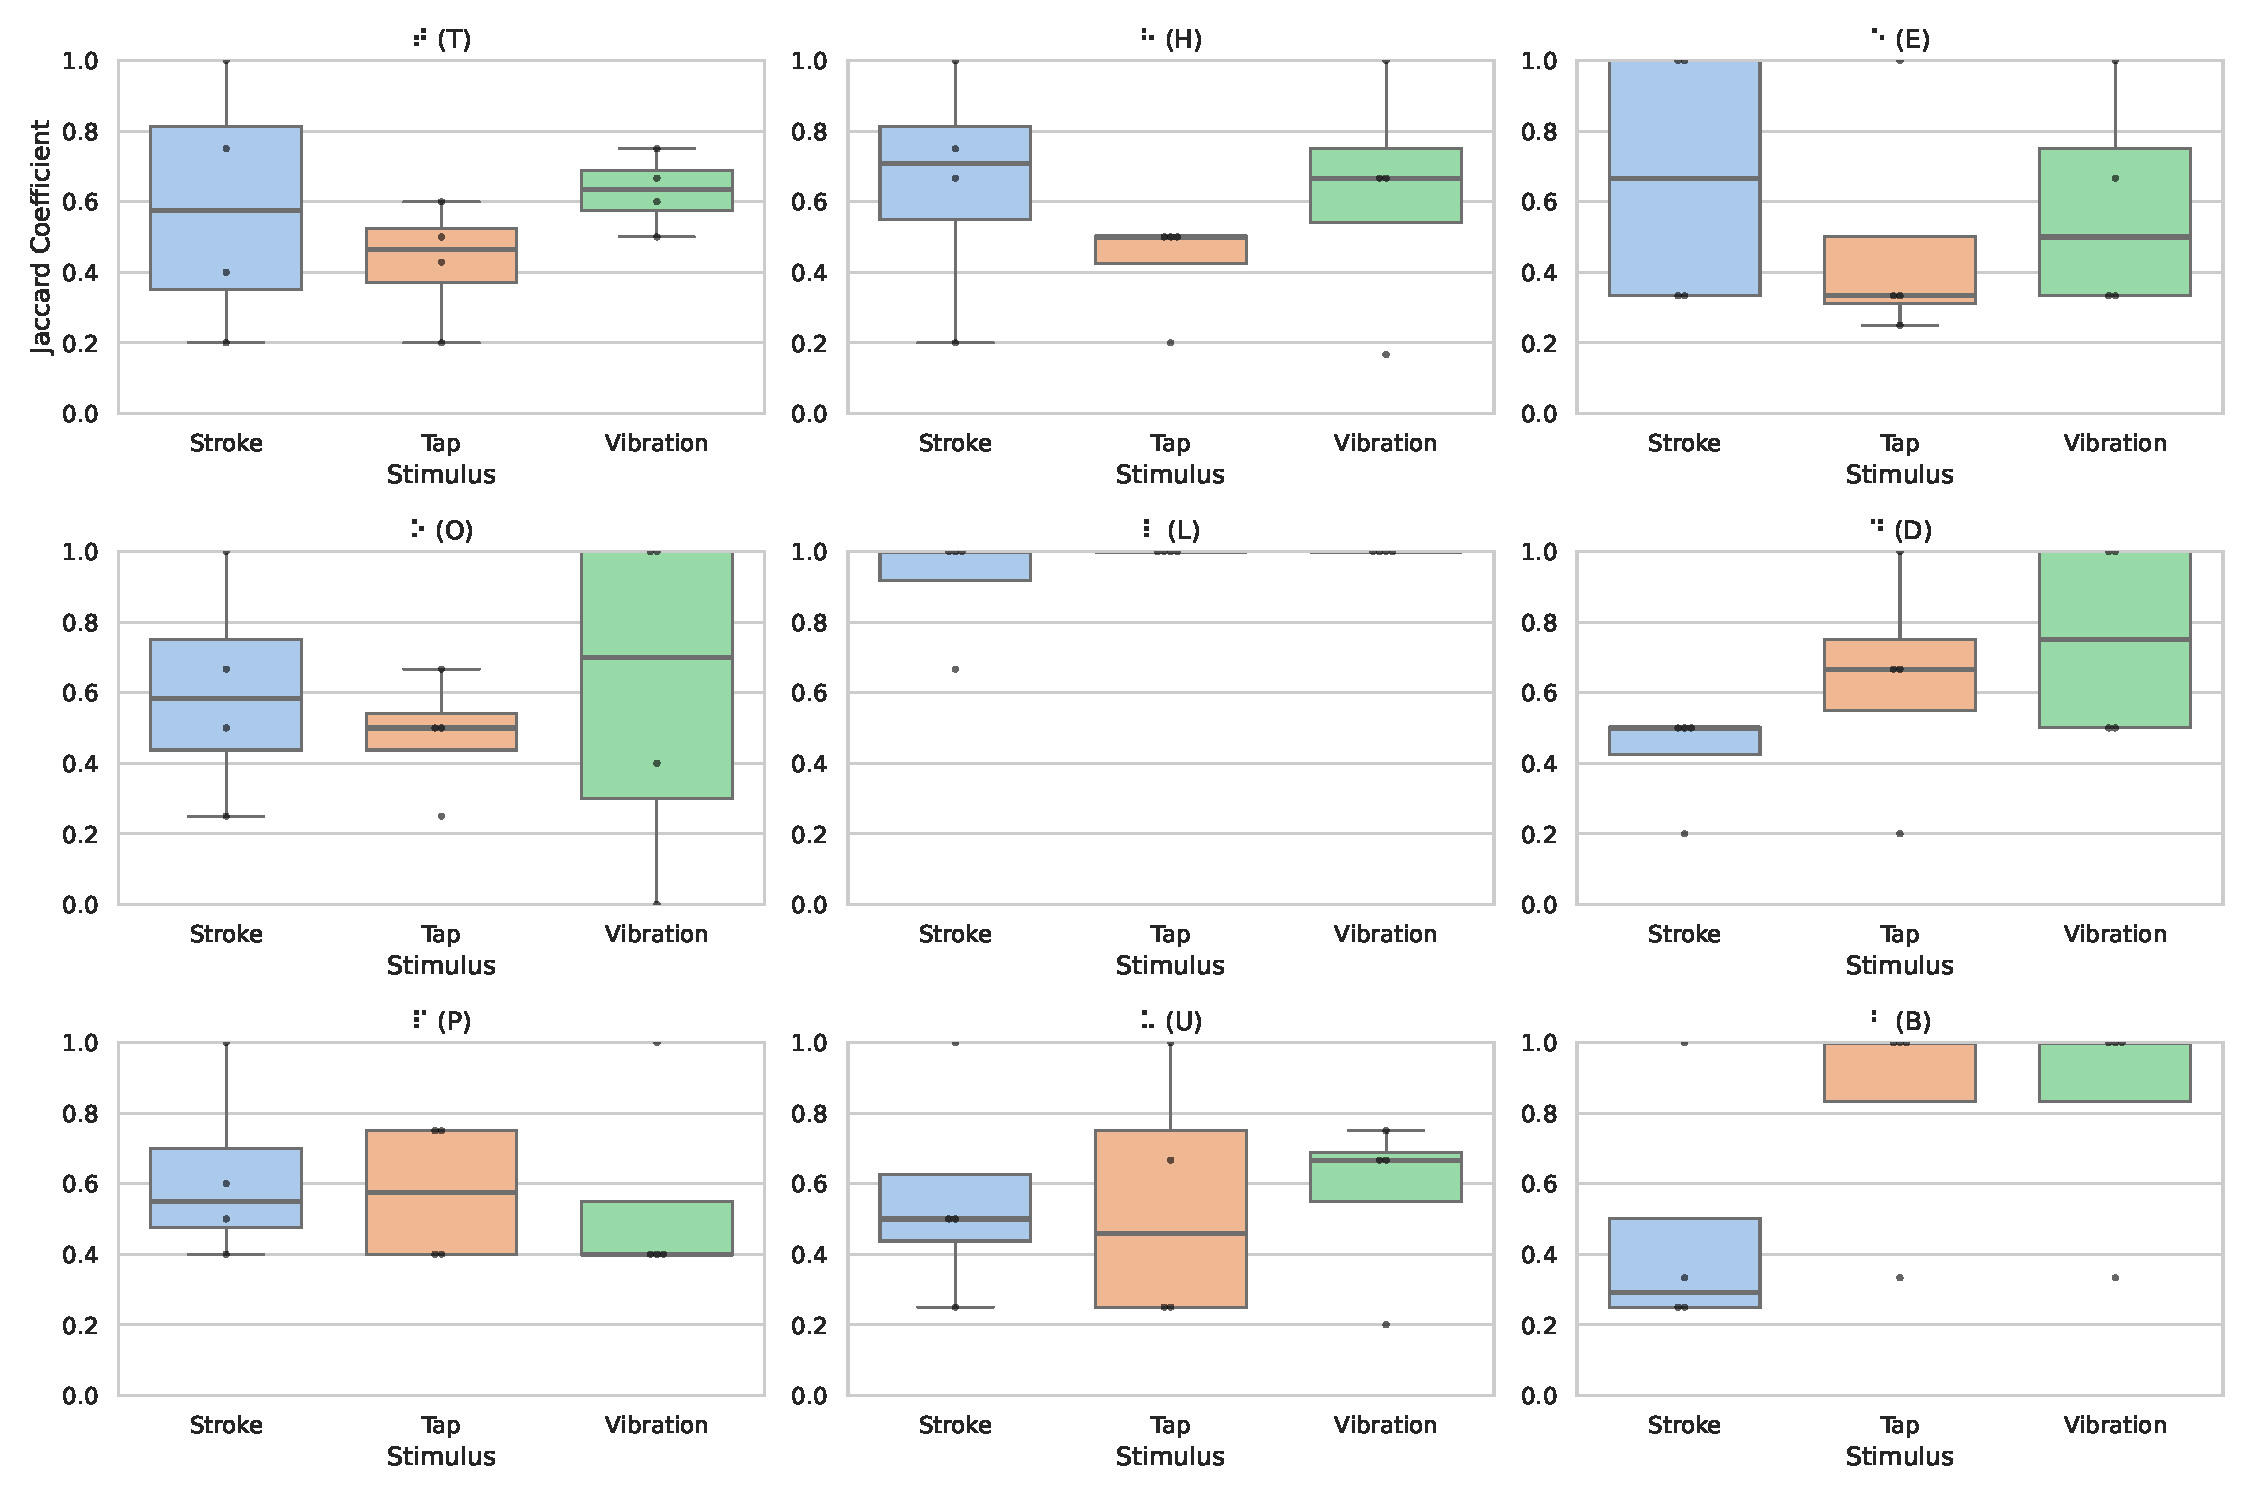
\includegraphics[width=\linewidth]{src/pictures/Study1Data_Experiment/Test_single_char.pdf}
    \caption{Jaccard coefficient results grouped by the Braille character during learning  for the different stimuli.\\Each dot represents one participant.}
    \label{fig:learning_results_firstStudy}
\end{figure}

After passively learning a character using a specific stimulus, a test was conducted to assess the performance of the characters immediately following the learning session. 
The test results are shown in \autoref{fig:learning_results_firstStudy}, where the stimuli are plotted with their respective Jaccard indices, grouped by the specific characters learned in the session.

The most significant difference is observed for the character \braille{b}(B), where the median for stroking is 0.3, while the medians for tapping and vibration are 1. The quantile ranges for tapping and vibration are 0.82 to 1, while the quantile range for stroking is 0.25 to 0.5.
As can also be seen, one of the outliers for stroke is one, and there were also one outlier for tapping and vibration respectively at 0.32.

A similar trend is observed for the character \braille{l}(L), where both tapping and vibration perform perfectly while stroking has an outlier at 0.675 and a lower q1 at 0.925 compared to the other ones at 1. However, all medians are the same at 1.

For the character \braille{h}(H), a larger difference is evident between tapping and the other two stimuli. While tapping has a median of 0.5, the medians for the other two stimuli are approximately 0.7. All three stimuli had a poor outlier, with a score of 0.2.

Another notable difference in medians appears for the character \braille{d}(D), where the median for stroking is 0.5, compared to medians of 0.675 for tapping and 0.75 for vibration. Additionally, the quantile ranges differ: vibration has the largest range, from 0.5 to 1, due to two participants scoring 0.5 and 1, respectively. In contrast, only one participant achieved a perfect score for tapping, and both tapping and stroking have worse participant scores of 0.2.

A further difference can be observed for the character \braille{t}(T), where the median for stroking is approximately 0.6, 0.65 for vibration, and 0.475 for tapping.

To test for significance, we used the Kruskal-Wallis tests, as none participant was tested twice on the same character. The results, however, did not show any significant differences, as depicted in \autoref{table:learning_significance_results_firstStudy_nonParam_learning}. 
As shown in the \enquote{p-value} column, all p-values for the tests exceed the threshold value of $\alpha = 0.05$, indicating no statistically significant difference between the Jaccard index results of the stimuli for any of the characters.


\begin{table}[ht]
\resizebox{\columnwidth}{!}{
\centering
\begin{tabular}{|l|l|l|l|l|}
\hline
\textbf{Question} & \textbf{Test Statistic} & \textbf{p-value}  &\textbf{Significance}           &\textbf{Effect Size}\\ \hline
\braille{t}(\textbf{T})& 1.9406 & 0.3790  &Not Significant &0.1764\\ \hline
\braille{h}(\textbf{H})& 2.2817& 0.3195&Not Significant &0.2074\\ \hline
\braille{e}(\textbf{E})& 1.1068 & 0.5750  &Not Significant &0.1006\\ \hline
\braille{o}(\textbf{O})& 0.2790& 0.8698&Not Significant &0.0254\\ \hline
\braille{l}(\textbf{L})& 2.0000 & 0.3679  &Not Significant &0.1818\\ \hline
\braille{d}(\textbf{D})& 2.9298& 0.2311&Not Significant &0.2663\\ \hline
\braille{p}(\textbf{P})& 0.7068 & 0.7023  &Not Significant &0.0643\\ \hline
\braille{u}(\textbf{U})& 0.0299& 0.9852&Not Significant &0.0027\\ \hline
\braille{b}(\textbf{B})& 3.6667 & 0.1599  &Not Significant &0.3333\\ \hline
\end{tabular}}
\caption{Results of Kruskal-Wallis significance tests for the different Braille characters during learning with a $\eta^2$ Effect Size.}
\label{table:learning_significance_results_firstStudy_nonParam_learning}
\end{table}



\begin{figure}
    \centering
    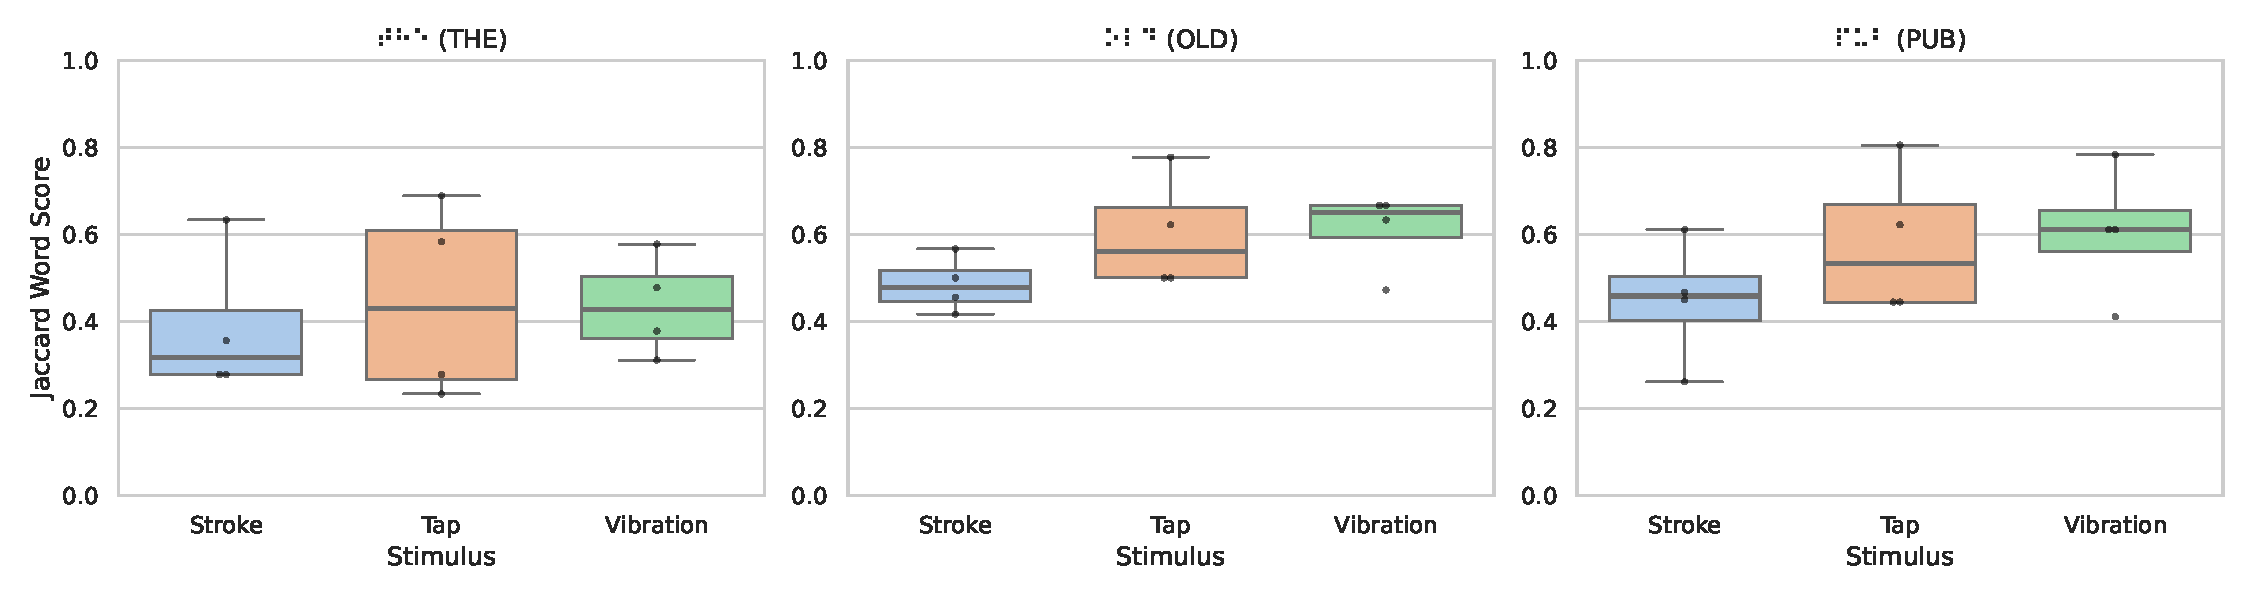
\includegraphics[width=\linewidth]{src/pictures/Study1Data_Experiment/JaccardTest.pdf}
    \caption{Jaccard Word-Test results grouped by the results for the Braille test-words\\
    \enquote{THE}, \enquote{OLD} and \enquote{PUB} for different stimuli.}
    \label{fig:test_results_firstStudy}
\end{figure}



After the passive learning sessions for all characters using a single stimulus, we conducted a word test for the characters learned during the previous passive learning sessions with that stimulus. 
The Jaccard score results, compared across the stimuli for each word, are depicted in \autoref{fig:test_results_firstStudy}. 
As shown, the differences in the Jaccard results are smaller than those observed for the individual characters. 

For the word \braille{the}(THE), the medians are 0.375 for stroking, 0.425 for tapping, and 0.425 for vibration. The quantile ranges are 0.35-0.5 for stroking, 0.3-0.6 for tapping, and 0.475-0.45 for vibration, respectively.

For the word \braille{old}(OLD), the medians are 0.62 for tapping and 0.625 for vibration, compared to 0.475 for stroking.

For the word \braille{pub}(PUB), the median for stroking (0.45) is somewhat lower than that for tapping (0.56) and vibration (0.61). 

Additionally, it can be observed that the quantile range for tapping is almost twice as large as that of the other two stimuli, with an approximate range of 0.2 compared to 0.1 for both vibration and stroking.

To test for significance, we performed a Kruskal-Wallis test, the results of which are depicted in \autoref{table:significance_results_test_firstStudy}. 
The results showed that all p-values are well above the threshold $\alpha$, with the closest value being 0.1371 for the word \braille{old}(OLD). 
This indicates that there was no statistically significant difference between the Jaccard index results for the different stimuli in relation to the word tests.

\begin{table}[ht]
\resizebox{\columnwidth}{!}{
\centering
\begin{tabular}{|l|l|l|l|l|}
\hline
\textbf{Question} & \textbf{Test Statistic} & \textbf{p-value}  &\textbf{Significance}           &\textbf{Effect Size}\\ \hline
\braille{the}(\textbf{THE})& 0.0361& 0.9821&Not Significant &0.0036\\ \hline
\braille{old}(\textbf{OLD})& 3.9736 & 0.1371  &Not Significant &0.1371\\ \hline
\braille{pub}(\textbf{PUB})& 1.0569& 0.5895&Not Significant &0.0961\\ \hline
\end{tabular}}
\caption{Results of the Kruskal-Wallis significance tests for the wordtests \enquote{THE}, \enquote{OLD}, and \enquote{PUB} with a $\eta^2$ Effect Size.}
\label{table:significance_results_test_firstStudy}
\end{table}



\begin{figure}
    \centering
    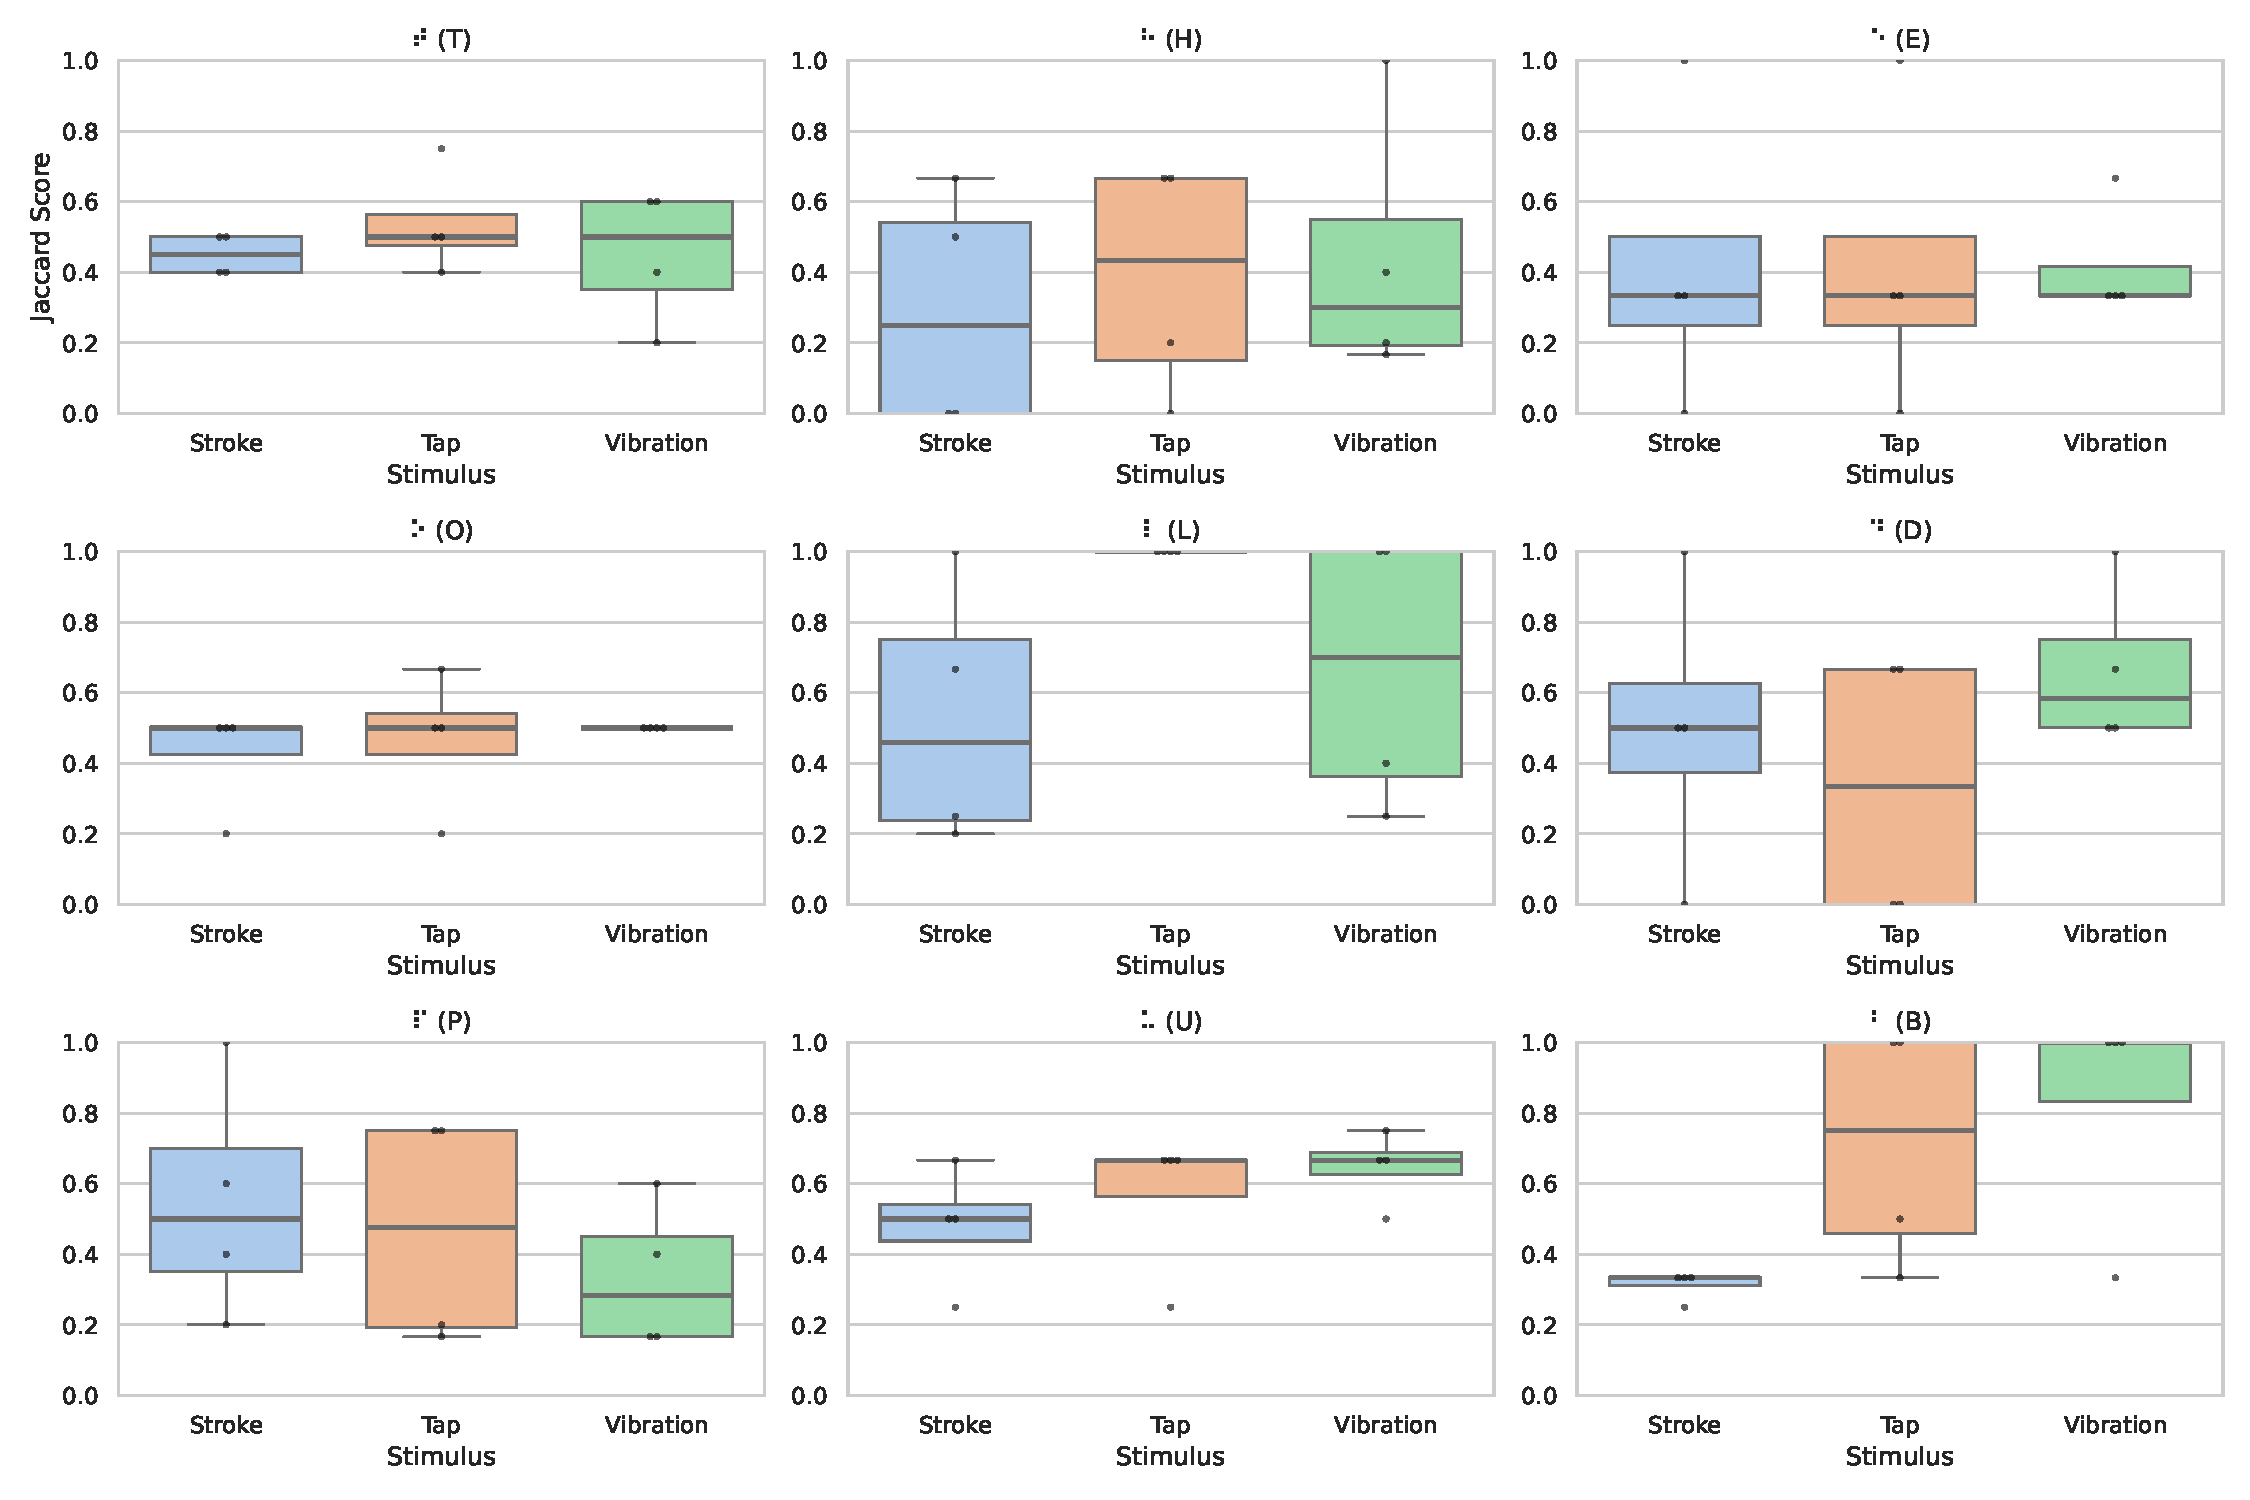
\includegraphics[width=\linewidth]{src/pictures/Study1Data_Experiment/boxplot_with_swarm_single_chars_test.pdf}
    \caption{Jaccard Score comparison for the different Stimuli grouped by the Braille test-word characters.}
    \label{fig:jaccard_test_study1}
\end{figure}


We further investigated the results by breaking them down for each individual character and analyzing them by examining false positives and false negatives in the construction of the Jaccard score. 
We regarded the decision to press a key or not as a classification task. 
Thus, a "missed character" is classified as a false negative, and a "surplus character" is classified as a false positive. 
Using this approach, we calculated precision and recall to derive the Jaccard score. 
These values are plotted in \autoref{fig:jaccard_test_study1}. 

As shown in the plot, the Jaccard score values do not differ significantly across most of the boxplots. 
The largest differences are observed for the character \braille{l}(L), where tapping performed the best with a median of 1 while stroking performed the worst with a median of 0.45 and vibration had a median of 0.7. 
Although perfect scores are observed for all stimuli, stroking had more \enquote{low performers}, with Jaccard scores of 0.2 and 0.25.

The character \braille{b}(B) showed a different pattern, with a median of approximately 0.325 for stroking, 0.75 for tapping, and 1 for vibration. 
None of the stroking participants were able to press the correct keys, whereas 2 participants in the tapping condition and 3 in the vibration condition succeeded in learning the character.

Additional differences were noted for the characters \braille{d}(D) and \braille{p}(P). 
For \braille{p}(P), the median for stroking was higher than the other stimuli, with a median of 0.5 compared to 0.45 for tapping and 0.3 for vibration. 

For \braille{d}(D), stroking was the worst-performing stimulus, with a median of 0.5 compared to 0.6 for tapping and 0.58 for vibration. 
It is important to note that there was only one perfect score for both vibration and stroking, while there were also scores of 0 for both stroking and tapping.

However, when testing for statistical significance using Kruskal-Wallis tests, which are tabulated in \autoref{table:learning_significance_results_firstStudy_nonParam}, no significant differences were found for any stimulus across the characters, with the exception of \braille{b}(B), which approached significance with a p-value of 0.0559 and a large \(\eta^2\) effect size of 0.3906.


\begin{table}[ht]
\resizebox{\columnwidth}{!}{
\centering
\begin{tabular}{|l|l|l|l|l|}
\hline
\textbf{Question} & \textbf{Test Statistic} & \textbf{p-value}  &\textbf{Significance}           &\textbf{Effect Size}\\ \hline
\braille{t}(\textbf{T})& 1.0203& 0.6004&Not Significant &0.1131\\ \hline
\braille{h}(\textbf{H})& 0.0136& 0.9932&Not Significant &0.0017\\ \hline
\braille{e}(\textbf{E})& 0.0979& 0.9522&Not Significant &0.0121\\ \hline
\braille{o}(\textbf{O})& 0.5309& 0.7669&Not Significant &0.0622\\ \hline
\braille{l}(\textbf{L})& 3.3764& 0.1849&Not Significant &0.2968\\ \hline
\braille{d}(\textbf{D})& 0.5290& 0.7676&Not Significant &0.0620\\ \hline
\braille{p}(\textbf{P})& 1.6124& 0.4465&Not Significant &0.1519\\ \hline
\braille{u}(\textbf{U})& 2.5488& 0.2796&Not Significant &0.2207\\ \hline
\braille{b}(\textbf{B})& 5.7683& 0.0559&Not Significant &0.3906\\ \hline
\end{tabular}}
\caption{Results of Kruskal-Wallis significance tests for the different Braille characters during testing with a $\eta^2$ Effect Size.}
\label{table:learning_significance_results_firstStudy_nonParam}
\end{table}





\begin{figure}
    \centering
    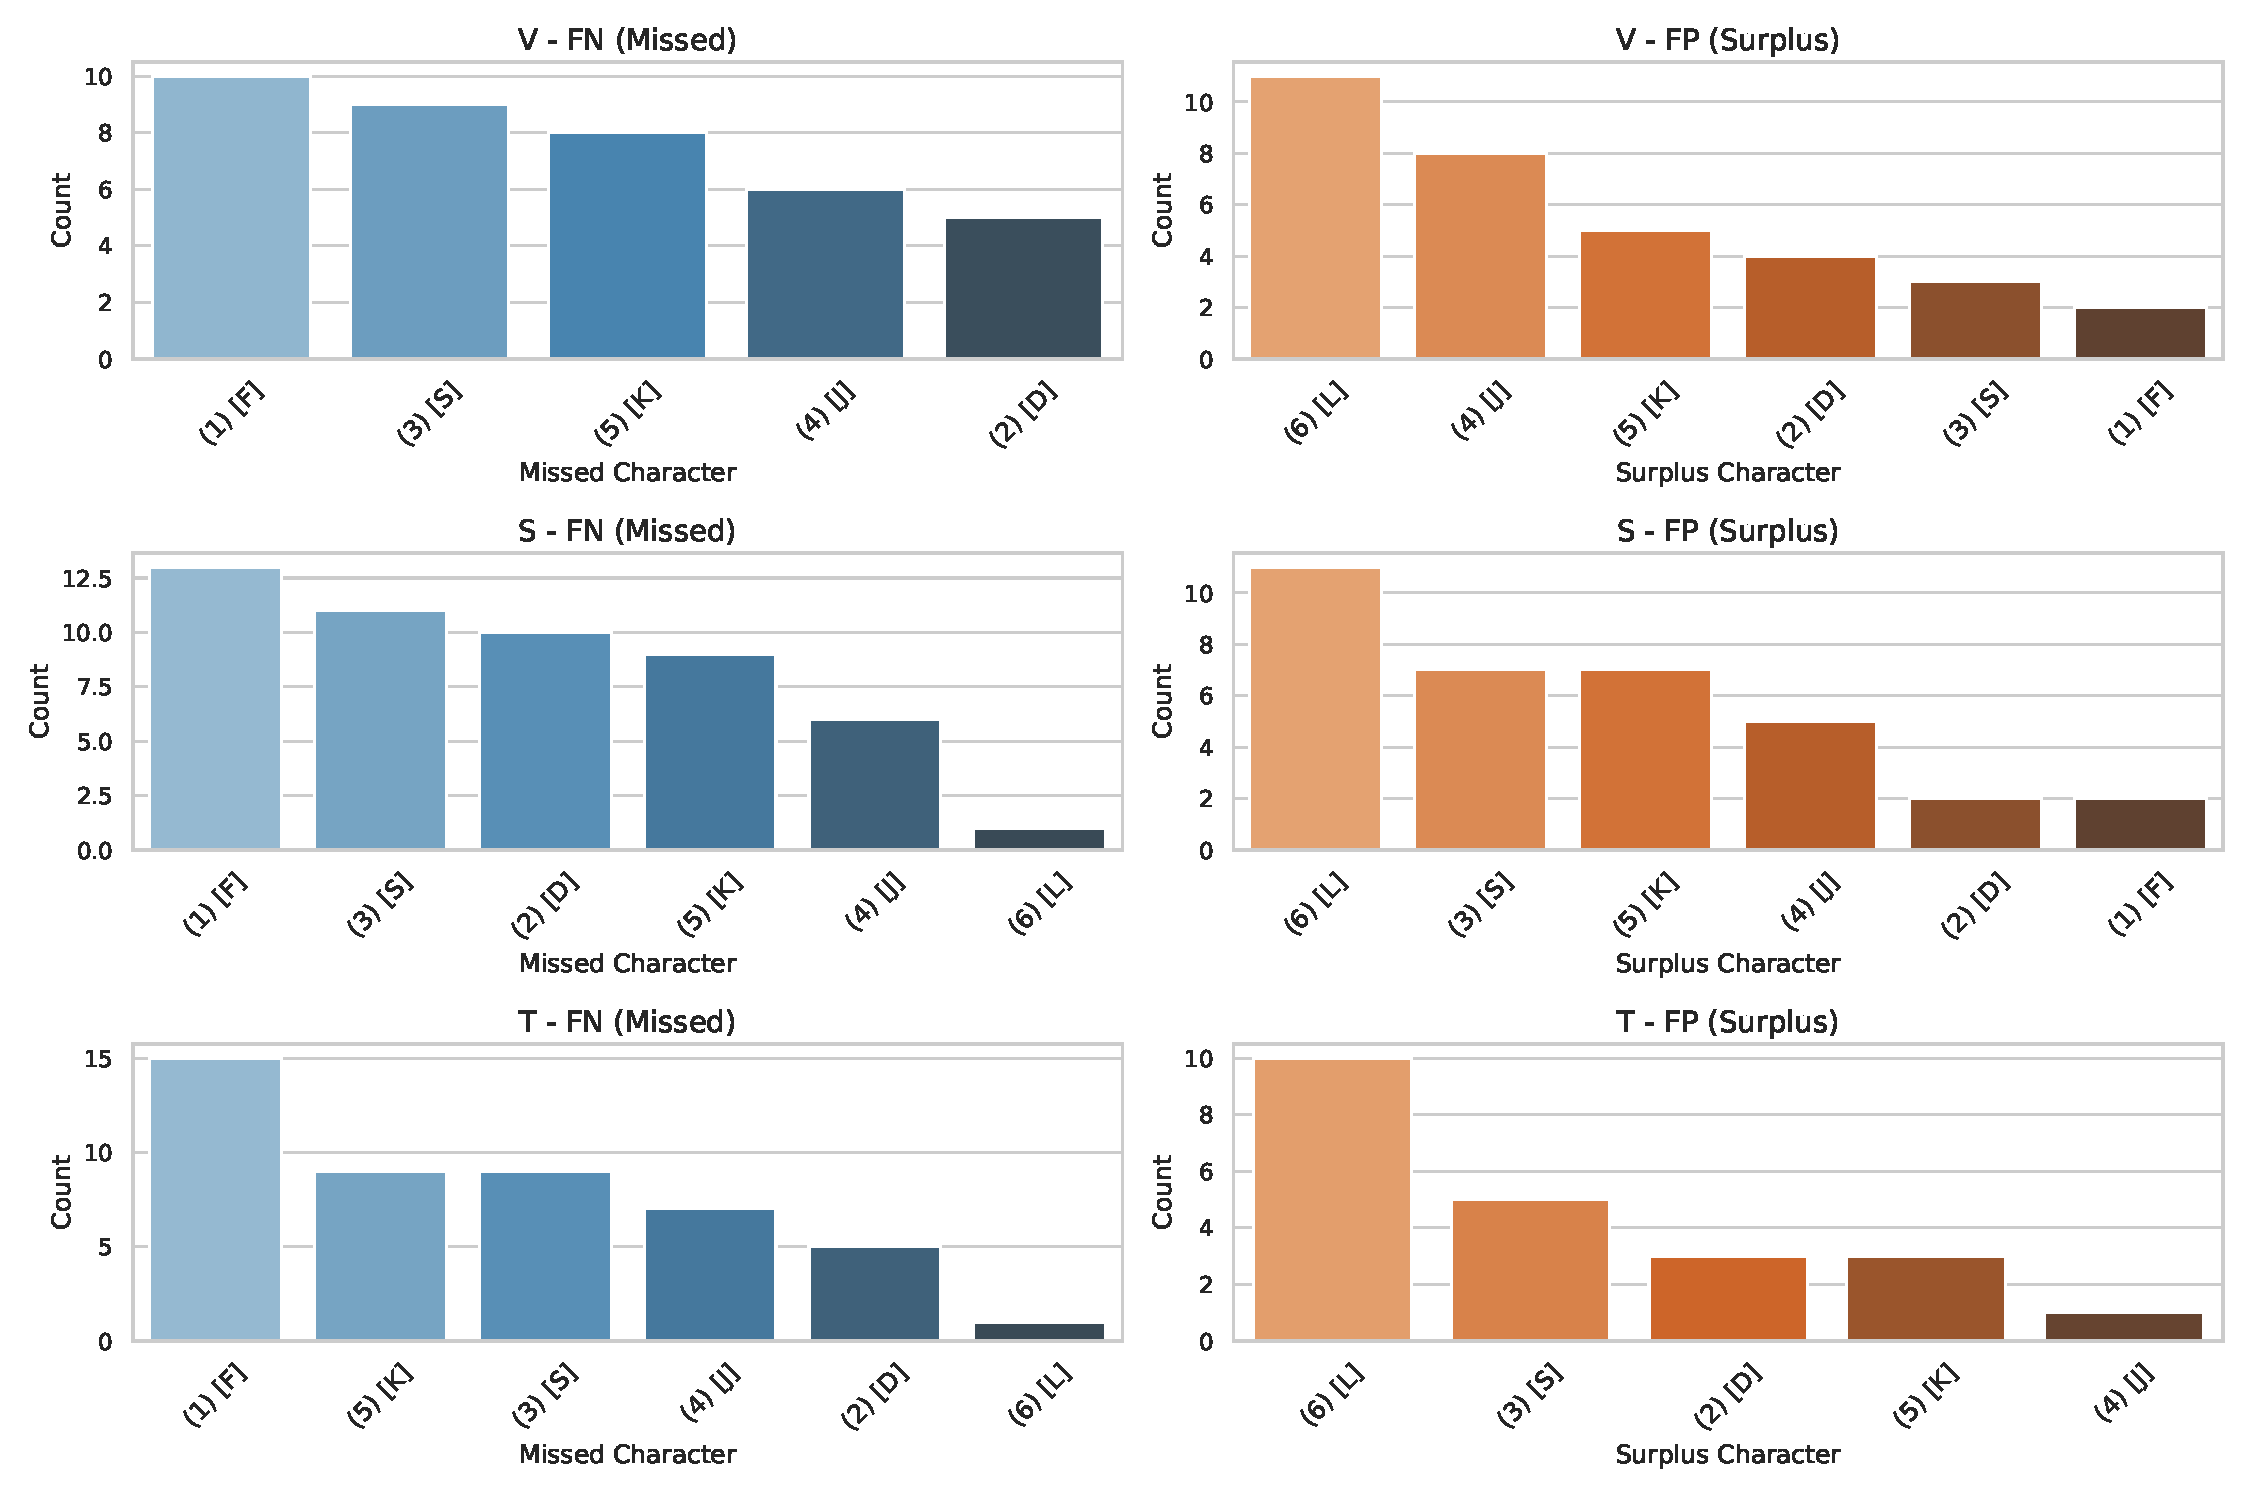
\includegraphics[width=\linewidth]{src/pictures/Study1Data_Experiment/columnChart.pdf}
    \caption{FN  (Missed) and FP (Surplus) key(s) for each stimuli.}
    \label{fig:missedSurplus_study1}
\end{figure}

To analyse the data that contributed to the Jaccard scores previously presented, we further examined the missed and surplus characters—those that were either missed or incorrectly submitted in addition to the required characters during the test. 
The results for the missed and surplus characters are depicted in \autoref{fig:missedSurplus_study1}, grouped by the stimulus.

As shown for the false negative characters (missed characters), marked in blue on the left side, the first two missed characters are always \textcircled{1} [F] and \textcircled{3} [S], followed by \textcircled{4} [K] for both the vibration and tapping stimuli. 
For the stroking stimulus, \textcircled{2} [D] follows, and then \textcircled{4} [K]. 
The character \textcircled{6} [L] was the least missed, as it does not appear among the missed characters for the vibration stimulus and ranks last for both the stroking and tapping stimuli. 
Next, the character \textcircled{2} [D] appears, which is ranked last for vibration and second-to-last for tapping. 
Following this, \textcircled{4} [J] is the second-to-last missed character for the vibration and stroking stimuli, and ranks third from the bottom for the tapping stimulus.

For the false positives (surplus characters), shown in red on the right, the most frequently added character is \textcircled{6} [L]. 
This indicates that, in most cases, the character \textcircled{6} [L] was added too often. However, the specific differences between the actuators vary. 
The \textcircled{1} [F] character appears last for the vibration stimulus, second-to-last for the stroking stimulus, and was never added as a surplus for the tapping stimulus.


\begin{figure}[h!]
    \centering
    \begin{subfigure}[b]{0.45\textwidth}
        \centering
        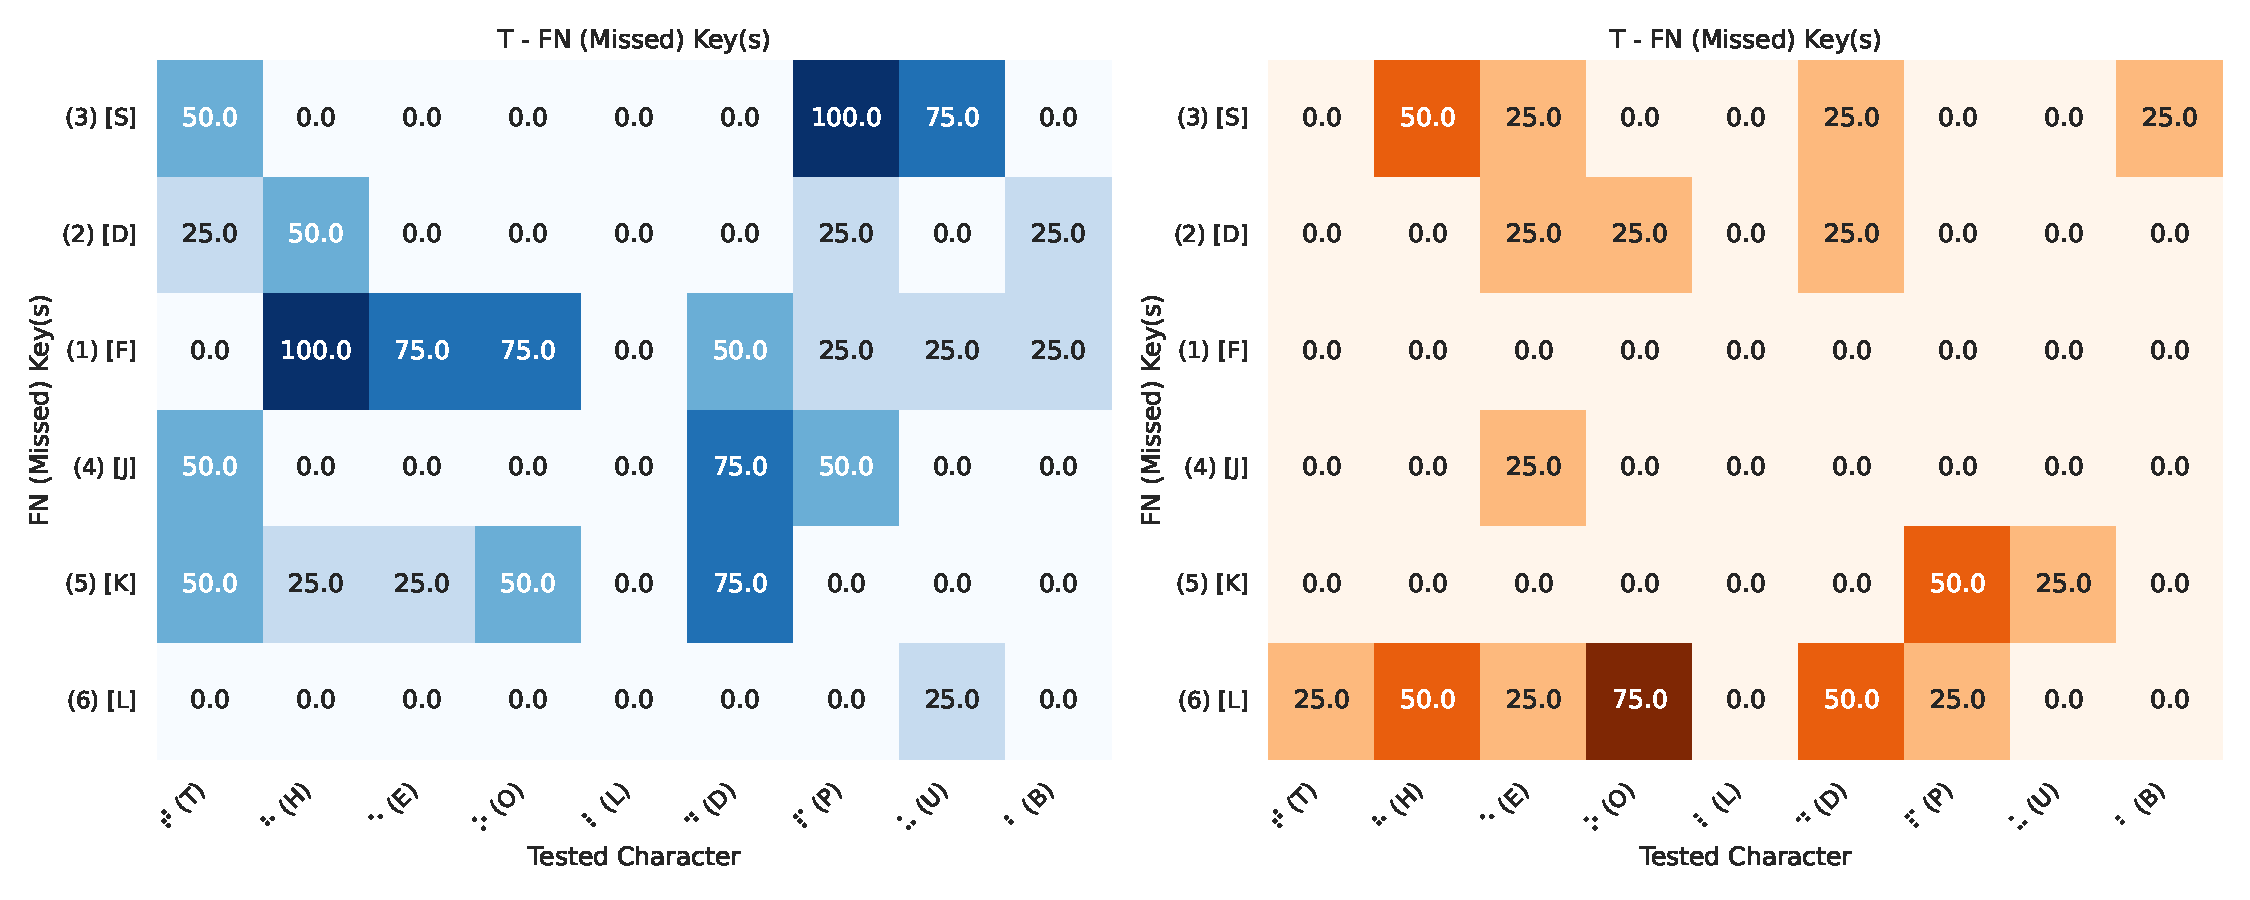
\includegraphics[width=\textwidth]{src/pictures/Study1Data_Experiment/heatmap_T_correlations_by_conditions_percentages.pdf}
        \caption{Tapping Stimulus}
    \end{subfigure}
    \begin{subfigure}[b]{0.45\textwidth}
        \centering
        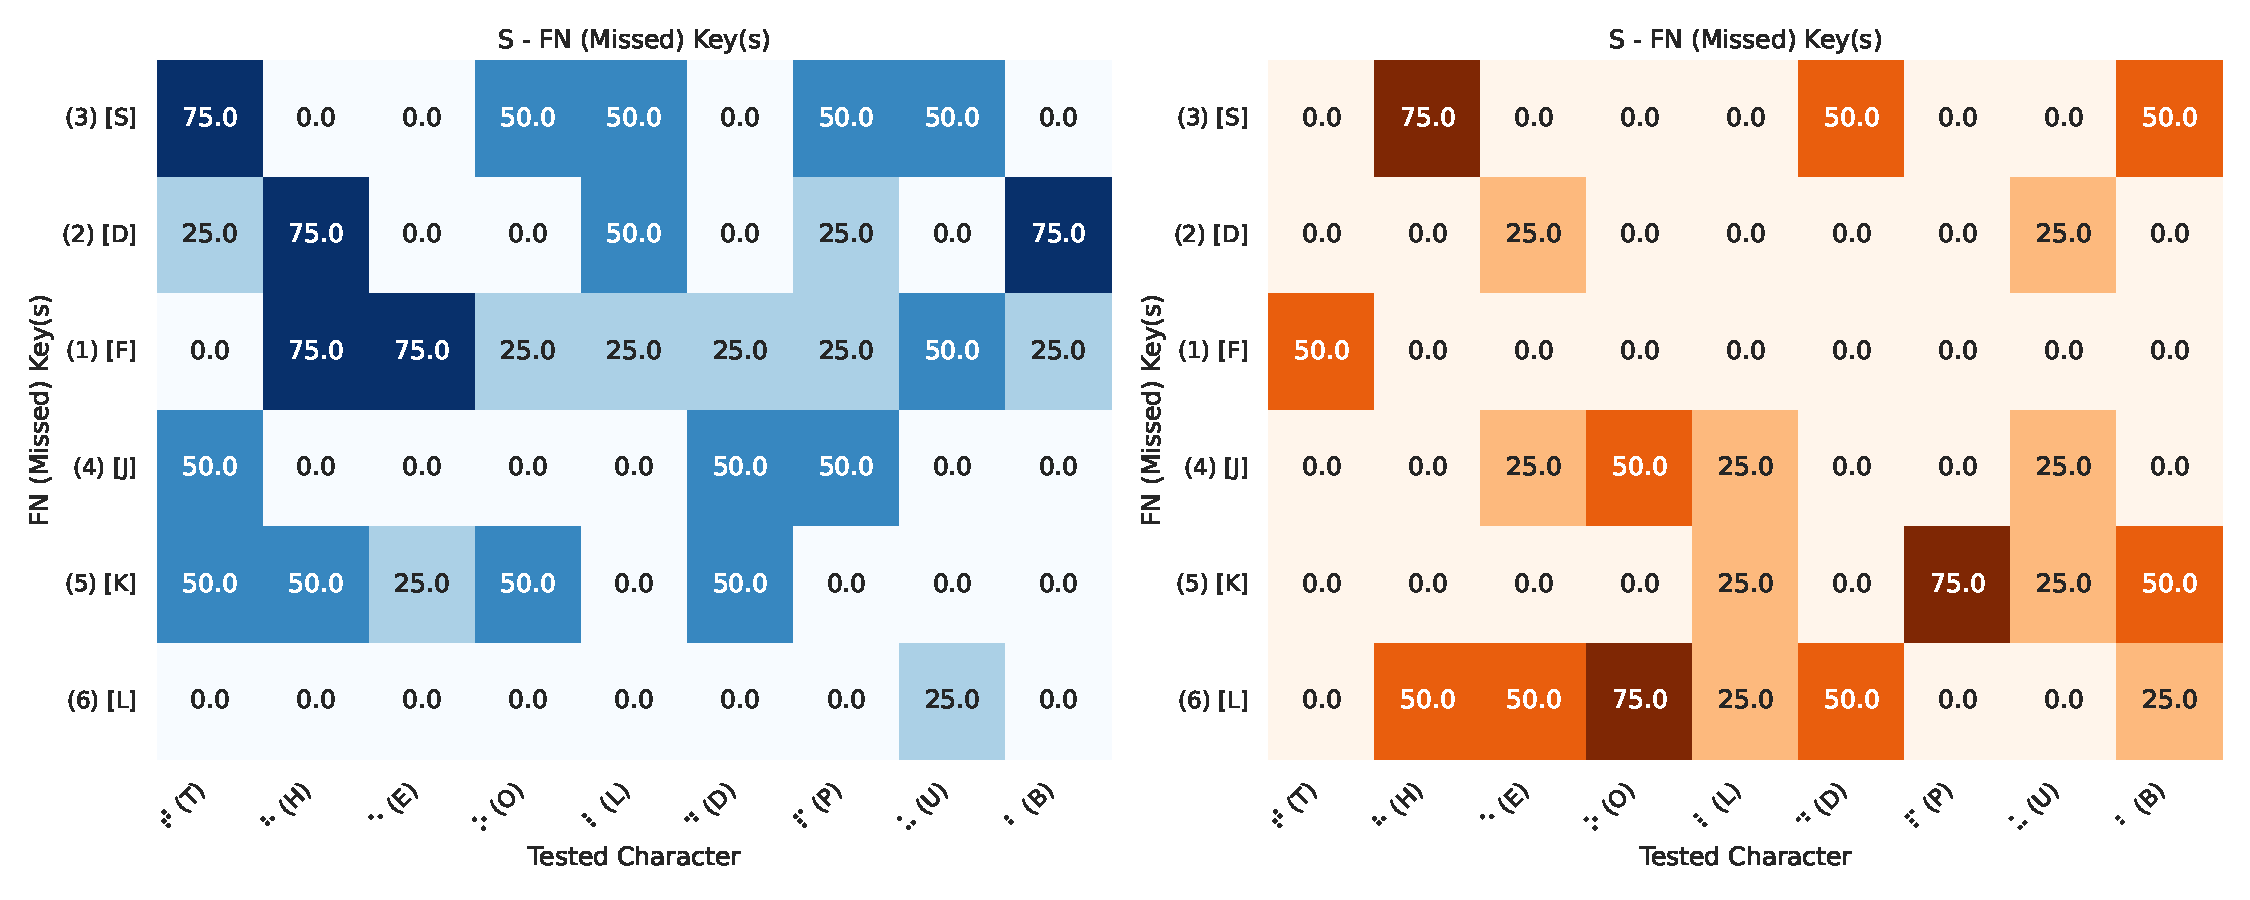
\includegraphics[width=\textwidth]{src/pictures/Study1Data_Experiment/heatmap_S_correlations_by_conditions_percentages.pdf}
        \caption{Stroking Stimulus}
    \end{subfigure}\\
    \begin{subfigure}[b]{0.45\textwidth}
        \centering
        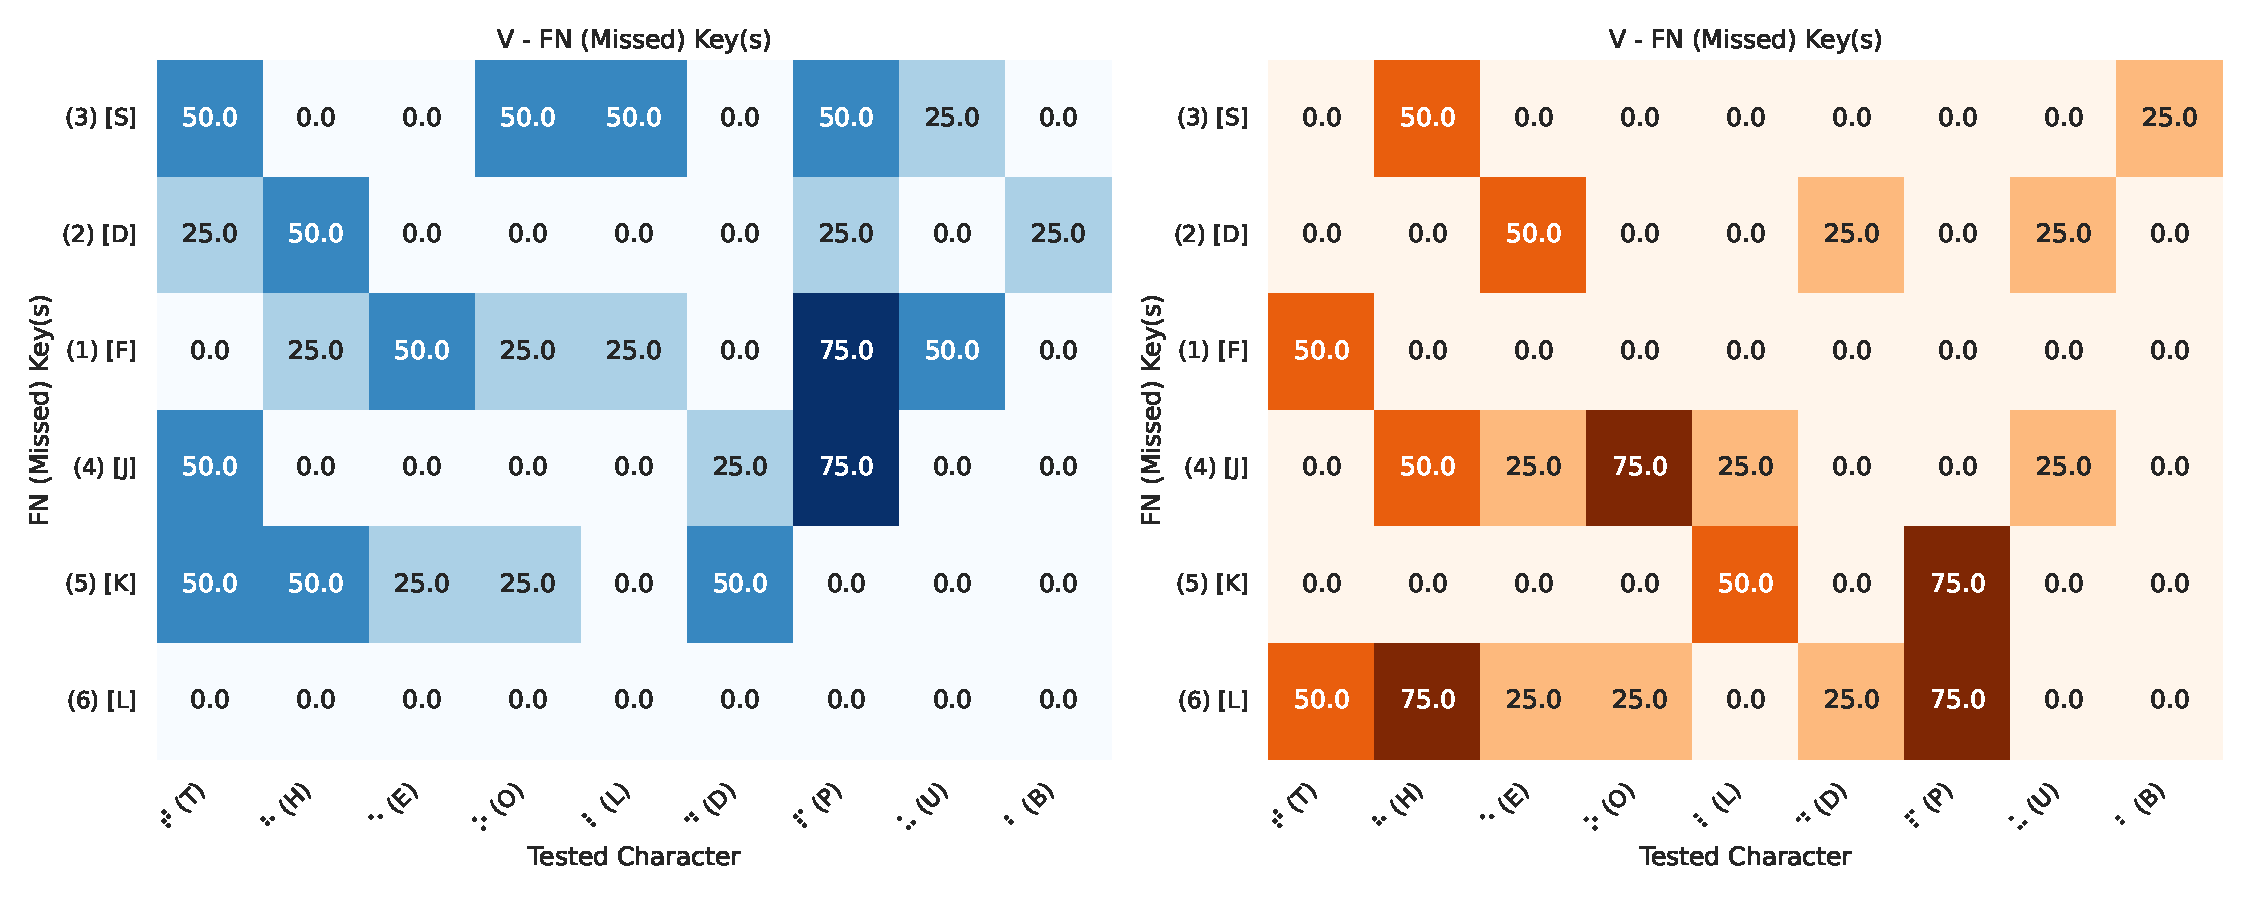
\includegraphics[width=\textwidth]{src/pictures/Study1Data_Experiment/heatmap_V_correlations_by_conditions_percentages.pdf}
        \caption{Vibration Stimulus}
    \end{subfigure}
    \caption{FN (Missed) Character in blue and FP (Surplus) keys in red in percent for each Braille character grouped by stimulus.}
    \label{fig:missed_surplus_percentages_study1}
\end{figure}

After analysing the missed and surplus characters, we now dive deeper into the specific relationships between each tested character and the corresponding surplus or missed character. These details are depicted in \autoref{fig:missed_surplus_percentages_study1}.

The diagram shows each Braille character under the category \enquote{tested character}, with the corresponding pressed keyboard characters on the left. 
The blue sections represent the percentage of missed keys when typing a character, while the red sections indicate surplus pressed keys for each character.

It is important to note that both \autoref{fig:missed_surplus_percentages_study1} and \autoref{fig:missedSurplus_study1} are related. Each column in \autoref{fig:missedSurplus_study1} corresponds to one row of missed or surplus characters in the same stimulus image, with matching colours for the same character. 
Thus, \autoref{fig:missed_surplus_percentages_study1} provides a more detailed, lower-level abstraction of the data shown in \autoref{fig:missedSurplus_study1}.

For the surplus (red) side, significant differences are observed for the Braille characters \braille{b}(B) and \braille{u}(U). For \braille{b}(B), the key \textcircled{3} [S] was consistently pressed incorrectly across all stimuli. However, for the Stroking stimulus, the keys \textcircled{5} [K] and \textcircled{5} [L] were also pressed incorrectly, with percentages of 50\% and 25\%, respectively.

Another notable difference occurs for the Braille character \braille{u}(U), where the key \textcircled{4} [K] was pressed incorrectly for the Tap and Stroking stimuli, and the keys \textcircled{4} [J] and \textcircled{2} [D] were pressed incorrectly for the Stroking and Vibration stimuli.

For the missed characters (FN, in blue), several differences are evident for the Braille characters \braille{l}(L) and \braille{b}(B). There were no missed characters for the Tapping stimulus, but for the Stroking and Vibration stimuli, the keys \textcircled{3} [S] and \textcircled{1} [F] were frequently missed. In the case of Stroking, the key \textcircled{2} [D] was missed in about 50\% of the trials.

A larger difference is seen with the key \textcircled{6} [L], which was never missed for the Vibration stimulus but was missed in about 25\% of cases for both the Stroking and Tapping stimuli.

\begin{figure}
    \centering
    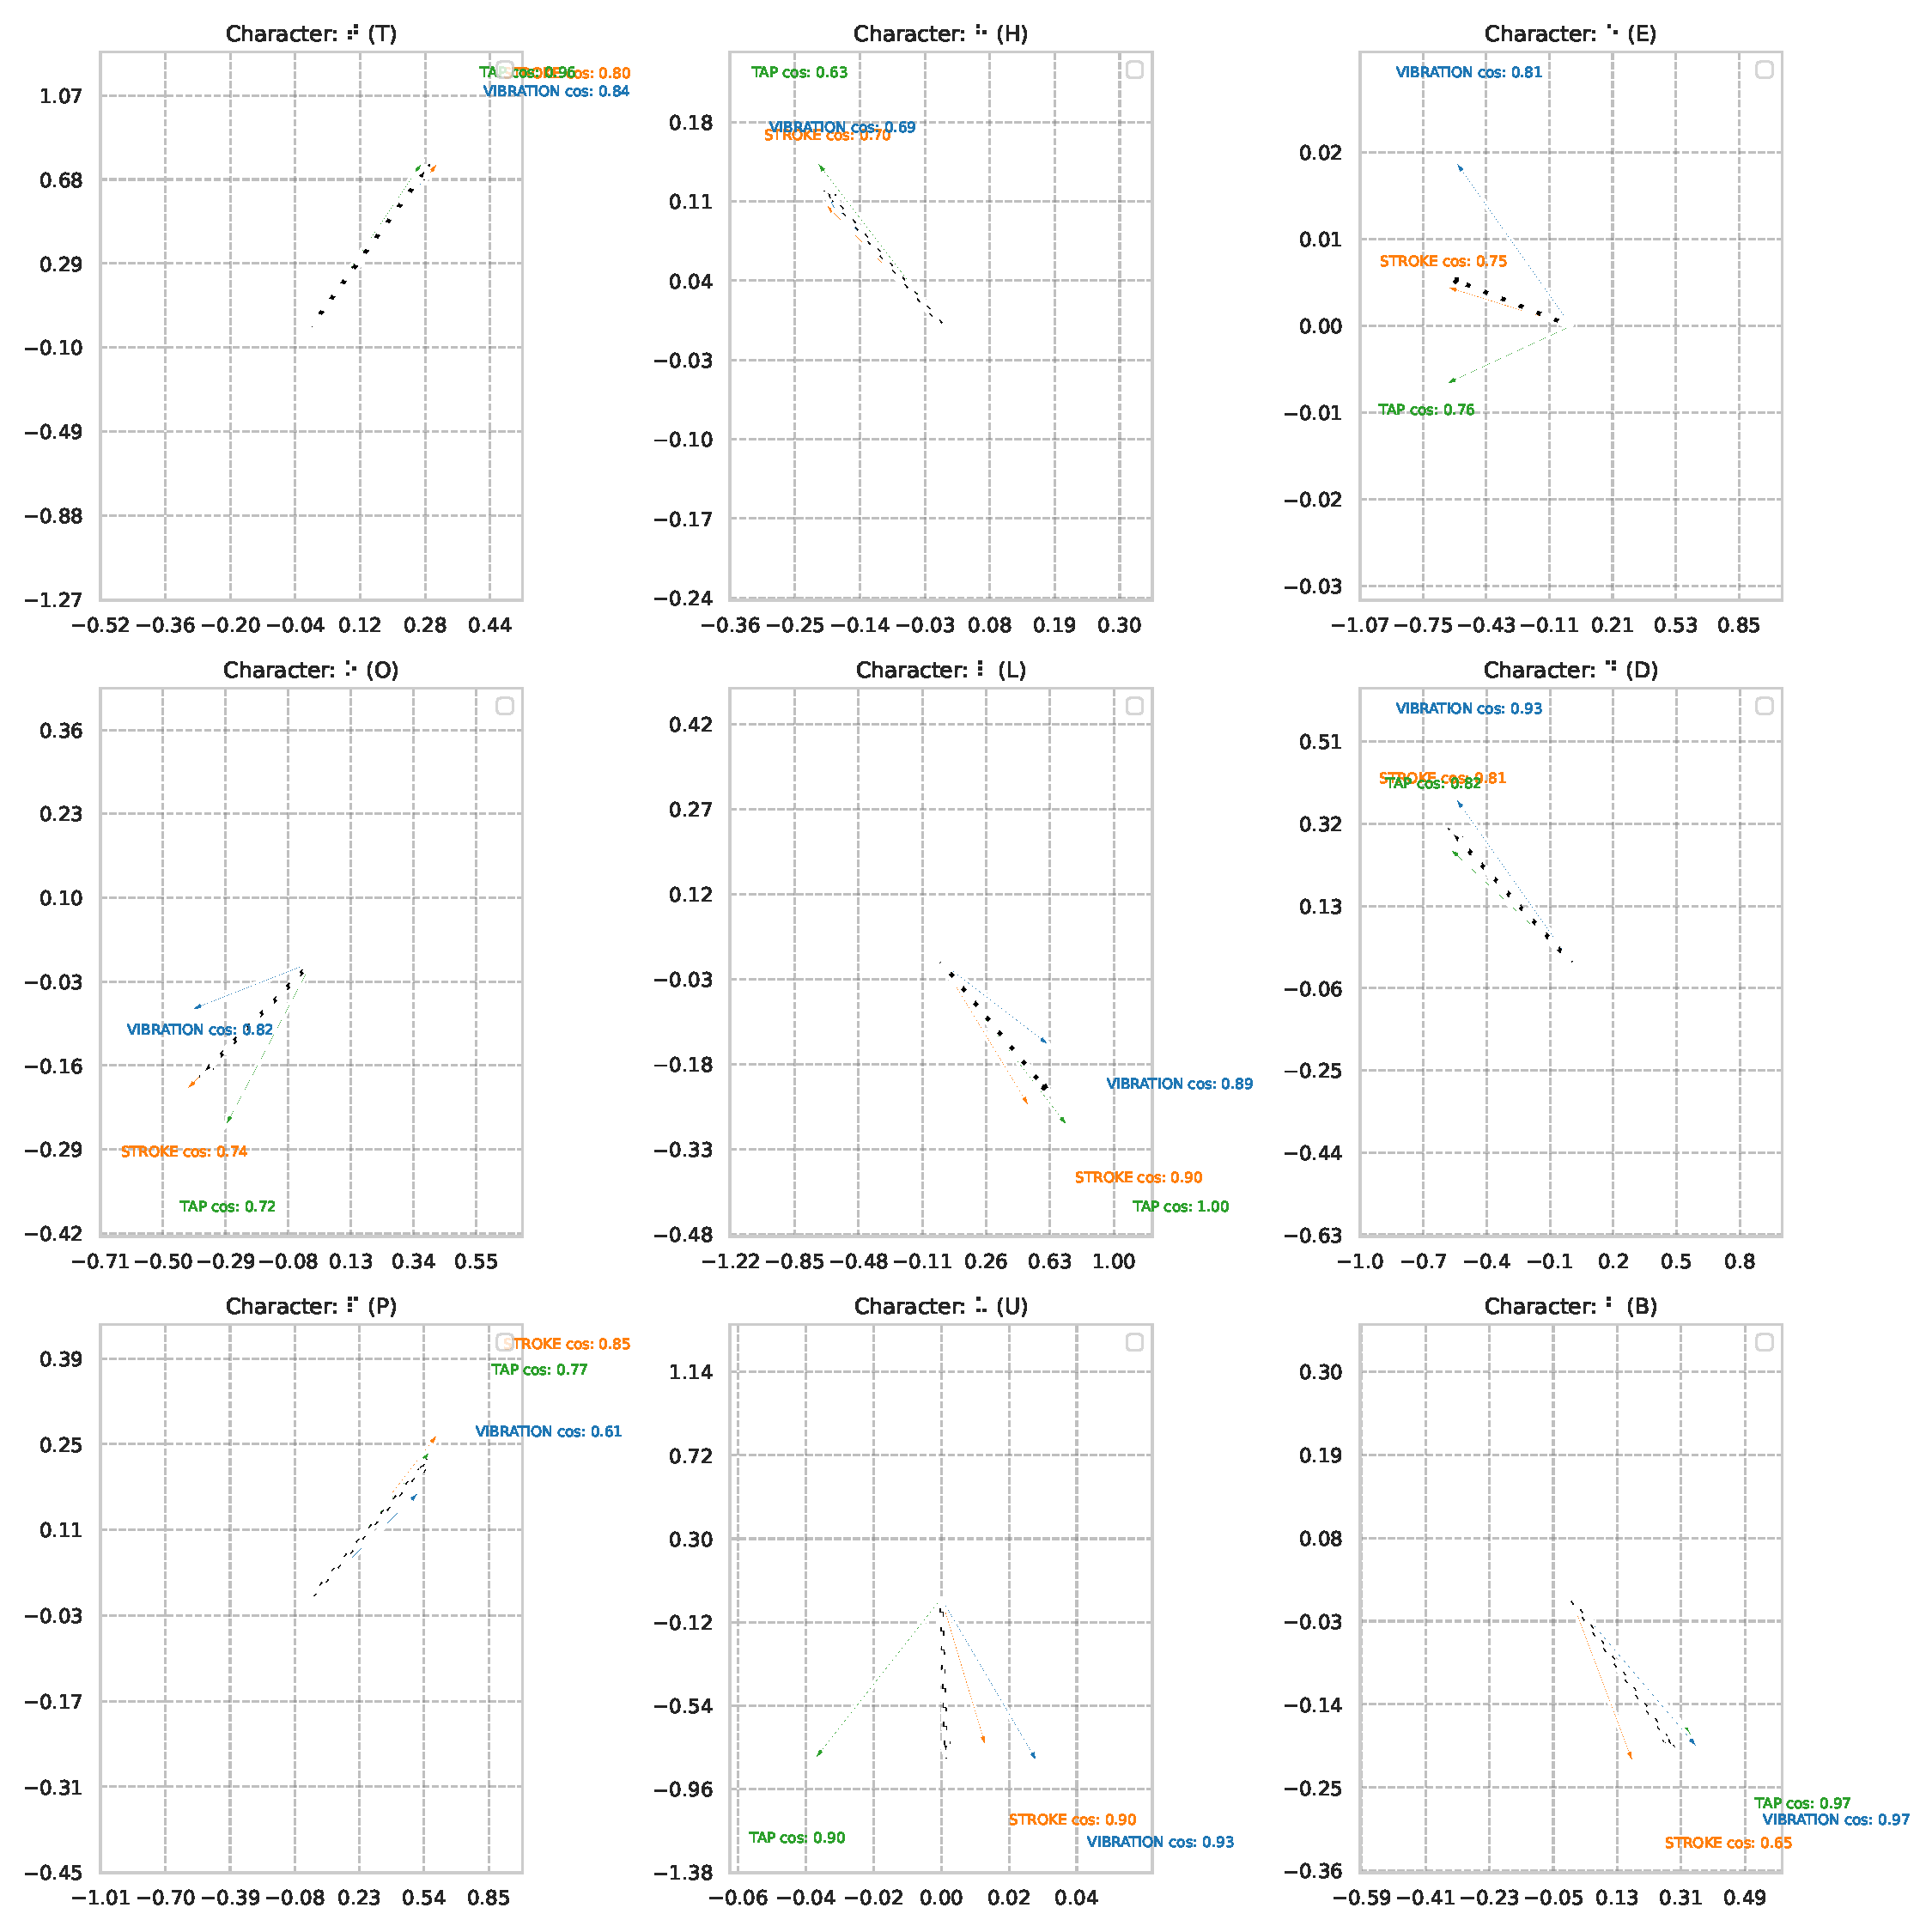
\includegraphics[width=\linewidth]{src/pictures/Study1Data_Experiment/Vectors_study1.pdf}
    \caption{Cosine Similariy for each of the Stimuli.\\Plotted using a \gls{pca} dimensionality reduction.}
    \label{fig:cosSim_PCA_study1}
\end{figure}

Lastly, a one-hot encoding vector was created for the pressed keys for each stimulus, similar to a column in \autoref{fig:missed_surplus_percentages_study1}. 
In order to visually represent the differences between the errors.
We then calculated the cosine similarity for each stimulus character vector embedding against the ground truth, which is depicted by the black dotted line in \autoref{fig:cosSim_PCA_study1}.
To present the cosine similarity in a visually appealing manner, we used \gls{pca} to reduce the dimensionality to two dimensions for plotting.

The cosine similarity and \gls{pca} analysis, as shown in the figure, indicate that despite noise reduction through \gls{pca}, the vectors align in a similar direction. The most noticeable differences were observed for the braille characters \braille{u}(U), \braille{e}(E), and \braille{o}(O).
But their Cosine similarity scores were still very similar with cosine scores of 0.81 (Vibration), 0.76 (Tapping) and 75 (Stroking) for the braille character \braille{e}(E), cosine scores of 0.82 (Vibration), 0.72 (Tapping) and 0.74 (Stroking) for the \braille{o}(O).
And lastly 0.9 (Tapping), 0.93 (Vibration) and 0.9 (Stroking) for the braille character \braille{u}(U)



\subsubsection{Questionnaire evaluation}
In our questionnaires we checked for correlations between each of the questions in order to check for hidden patterns of the participants.

\begin{table}[ht]
\resizebox{\columnwidth}{!}{
\centering
\begin{tabular}{|l|l|l|l|l|}
\hline
\textbf{First Question}& \textbf{Second Question}& \textbf{Tap} Pearson correlation r&\textbf{Stroke} Pearson correlation r &\textbf{Vibration} Pearson correlation r\\ \hline
Mental Demand& Effort& \textbf{0.67}&0.27&\textbf{0.56}\\\hline
\end{tabular}}
\caption{Correlation within the Nasa TLX dimensions.}
\label{table:nasaTLX_correlation_firstStudy}
\end{table}
% The table \autoref{table:nasaTLX_correlation_firstStudy} tabulates the \enquote{Mental Demand} dimension, which is the only one, that has an at least median average correlation over all the stimuli.
% As can be seen, the correlation is strong for the tapping, and moderate for vibration between \enquote{Mental Demand} and \enquote{Effort}, however, the stroke has a weak correlation with between the two dimensiosn, however, it is the only dimension, that is on average correlated over the stimuli.
The table \autoref{table:nasaTLX_correlation_firstStudy} presents the \enquote{Mental Demand} dimension, which is the only one with at least a median average correlation across all stimuli.
As shown, there is a strong correlation between \enquote{Mental Demand} and \enquote{Effort} for tapping, and a moderate correlation for vibration. In contrast, the stroke stimulus shows only a weak correlation between these two dimensions. Nevertheless, \enquote{Mental Demand} is the only dimension that, on average, correlates across all stimuli.


\begin{table}[ht]
\resizebox{\columnwidth}{!}{
\centering
\begin{tabular}{|l|l|l|l|l|}
\hline
\textbf{First Question}& \textbf{Second Question}& \textbf{Tap} Pearson correlation r&\textbf{Stroke} Pearson correlation r &\textbf{Vibration} Pearson correlation r\\ \hline
Physical Demand& Feeling Pleasant& -0.1&\textbf{-0.64}&\textbf{-0.7}\\\hline
 & Would use actuators to support the learning process& -0.32& \textbf{-0.63}&\textbf{-0.58}\\\hline
 Performance& Helped Learning& \textbf{-0.51}& 0.37&-0.41\\\hline
 & Would use actuators to support the learning process& -0.47& -0.19&\textbf{-0.66}\\\hline
 & Able to understand haptic feedback& \textbf{-0.51}& \textbf{-0.54}&\textbf{-0.69}\\\hline
 Frustration& Helped Learning& -0.42& -0.41&-0.4\\\hline
 & Able to understand haptic feedback& -0.43& -0.31&\textbf{-0.67}\\\hline
 & Satisfaction overall& -0.48& -0.26&\textbf{-0.58}\\\hline
\end{tabular}}
\caption{Correlation between the Nasa TLX and Usability questionnaire dimensions.}
\label{table:usability_correlation_firstStudy}
\end{table}
% For the usability table depicted in \autoref{table:usability_correlation_firstStudy}, that depictes all the dimension pairs, that have an at least medium correlation between the different stimuli.
% However, the only dimension pair, that has an at least medium correlation between all stimuli is between the \enquote{Performance} and \enquote{Able to understand haptic feedback} category, with correlation values of \textbf{-0.51} for tapping, \textbf{-0.54} for stroking and \textbf{-0.69} for vibration, which shows that when their perceived performance was higher, their ability to understand haptic feedback was lower and vice versa with a medium correlation.

The usability table shown in \autoref{table:usability_correlation_firstStudy} lists all dimension pairs that exhibit at least a medium correlation across the different stimuli.
The only dimension pair that shows a medium or stronger correlation for all stimuli is between \enquote{Performance} and \enquote{Able to understand haptic feedback}, with correlation values of -0.51 for tapping, -0.54 for stroking, and -0.69 for vibration. This indicates a consistent inverse relationship: as participants perceived their performance to be higher, their ability to understand haptic feedback tended to be lower, and vice versa.


\begin{table}[ht]
\resizebox{\columnwidth}{!}{
\centering
\begin{tabular}{|l|l|l|l|l|}
\hline
\textbf{First Question}& \textbf{Second Question}& \textbf{Tap} Pearson correlation r&\textbf{Stroke} Pearson correlation r &\textbf{Vibration} Pearson correlation r\\ \hline
Helped Learning& Able to understand haptic feedback& \textbf{0.66}&0.17&\textbf{0.64}\\\hline
 & Would use actuators to support the learning process& 0.49& 0.26&\textbf{0.69}\\\hline
 & Satisfaction overall& \textbf{0.51}& \textbf{0.61}&\textbf{0.55}\\\hline
 Would use actuators to support the learning process& Would have learned faster& -0.47& \textbf{-0.63}&-0.19\\\hline
 & Able to understand haptic feedback& \textbf{0.71}& 0.47&\textbf{0.61}\\\hline
\end{tabular}}
\caption{Correlation within the Usability questionnaire dimensions.}
\label{table:questionnaire_correlation_secondStudy}
\end{table}
% When looking at the the usability questionnaire we also found some at least medium correlation for the averaged stimuli, which are depicted in \autoref{table:questionnaire_correlation_secondStudy}.
% One dimension pair is here especially important, the \enquote{Helped Learning} and \enquote{Satisfaction overall}, that shows that there is an at least median correlation for over the different stimuli with \textbf{0.51} for tapping, \textbf{0.61} for stroking and \textbf{0.55} for vibration.
% That shows that the satisfaction is correlated for the participants with the percieved improvement in learning for all of the stimuli.
The usability questionnaire also revealed several dimension pairs with at least medium correlations for the averaged stimuli, as shown in \autoref{table:questionnaire_correlation_secondStudy}.
One particularly noteworthy pair is \enquote{Helped Learning} and \enquote{Satisfaction overall}, which shows consistent medium correlations across all stimuli: 0.51 for tapping, 0.61 for stroking, and 0.55 for vibration.
This suggests that participants' overall satisfaction was positively associated with their perceived improvement in learning, regardless of the stimulus type.



\subsubsection{User comments}
The usability questionnaire also included an open-ended response field. Participants' comments were as follows:
\enquote{Stroking is better than vibration, and tapping is better than stroking in both comfort and learning.}
\enquote{For vibration, it is sometimes difficult to identify which finger is vibrating.}\footnote{Translated from: \enquote{Bei Vibration ist manchmal schwer zu finden, welche Finger vibriert.}}
\enquote{The vibration was unclear, as it was difficult to tell which fingers were vibrating due to interference from other vibrators. The stroking was hard to feel.}
\enquote{I think the tapping was the most comfortable, and I was able to distinguish the fingers. I sometimes couldn’t feel the stroker.}\footnote{Translated from: \enquote{Ich empfand den Tapper am angenehmsten und man konnte die Finger gut unterscheiden. Den Stroker habe ich manchmal nur kaum gespürt.}}
These responses consistently suggest that tapping was the most preferred stimulus, followed by stroking, and lastly vibration. Participants cited tapping’s comfort and finger distinguishability as advantages, while stroking was often described as difficult to feel and vibration as hard to localize due to interference.



% % \subsubsubsubsection{Task Load Assessment}

% In the first study, we evaluated participants’ perceived task load using the NASA TLX index. This index includes six dimensions: Mental Demand, Physical Demand, Temporal Demand, Performance, Effort, and Frustration. Statistical analysis revealed no significant differences between the stimuli across the six dimensions.

% However, an observable trend was noted in the \textit{Performance} dimension. The median scores suggest that participants perceived their performance more favorably under the stroking and vibration conditions. We hypothesize that this is due to a disconnect between actual and perceived performance—participants may have struggled to accurately identify the stimuli, leading to a more favorable self-assessment simply because they were unaware of their errors.

% % \subsection{Usability Questionnaire}

% The usability questionnaire revealed significant differences in two key dimensions: \textit{Overall Satisfaction} ($p = 0.0027$) and \textit{Would Have Learned Faster} ($p = 0.0104$), both with moderate Kendall's W effect sizes ($> 0.38$). An additional near-significant result was found for \textit{Helped Learning} ($p = 0.0701$), with a smaller effect size of approximately 0.22.

% These results suggest that participants were generally more satisfied with the tapping stimulus, and that both tapping and vibration stimuli contributed positively to the learning experience. Notably, participants reported that the vibration condition, more than tapping, gave them the impression they would learn faster.

% % \subsection{User Preference and Qualitative Feedback}

% When directly asked which stimulus was most helpful for learning, participants favored the tapping condition. Comfort ratings for tapping were also on par with the vibration stimulus, suggesting that tapping may strike a good balance between usability and comfort.

% Participant comments reinforce this finding. Examples include:

% \enquote{Stroking is better than vibration, and tapping is better than stroking in both comfort and learning.}
% \enquote{The vibration was unclear, as it was difficult to tell which fingers were vibrating due to interference from other vibrators. The stroking was hard to feel.}
% \enquote{I think the tapping was the most comfortable, and I was able to distinguish the fingers. I sometimes couldn’t feel the stroker.}

% Overall, participants preferred tapping, followed by stroking, and then vibration. The main issues cited were the indistinctness of vibration and the low perceptibility of stroking, while tapping was consistently noted as comfortable and easy to distinguish.

% % \subsection{Correlation Analysis}

% Correlation analysis revealed that the \textit{Performance} dimension was negatively correlated with participants' perceived ability to understand haptic feedback. This supports the idea that when participants felt they could clearly perceive the stimuli, they also became more aware of their errors—leading to a lower self-assessed performance.

% Additionally, there was a positive correlation between \textit{Helped Learning} and \textit{Overall Satisfaction}, suggesting that participants who found the stimuli helpful also reported higher satisfaction, likely due to better stimulus distinguishability.

% % \subsection{Learning Performance}

% Objective performance data from the word-learning tests did not show statistically significant differences across conditions. However, tapping and vibration stimuli tended to yield slightly better results in retention tasks. While not significant, this trend aligns with participants’ subjective assessments and indicates potential for further study.

% % \subsection{Conclusion}

% While no significant differences in overall task load were found between the stimuli, subjective responses provide strong support for the tapping and vibration stimulus. Tapping was rated highest in terms of satisfaction, learning support, and comfort, and participants found it easiest to distinguish. Vibration also showed promise, particularly in its perceived support for learning, though its comfort and clarity were less consistent. Stroking was the least preferred due to perceptual difficulties.


\subsection{Second Study}
\subsubsection{Evaluation of the experiment results}
We investigated the results more, and looked into what kind of errors and what errors are generated in general.

\begin{figure}
    \centering
    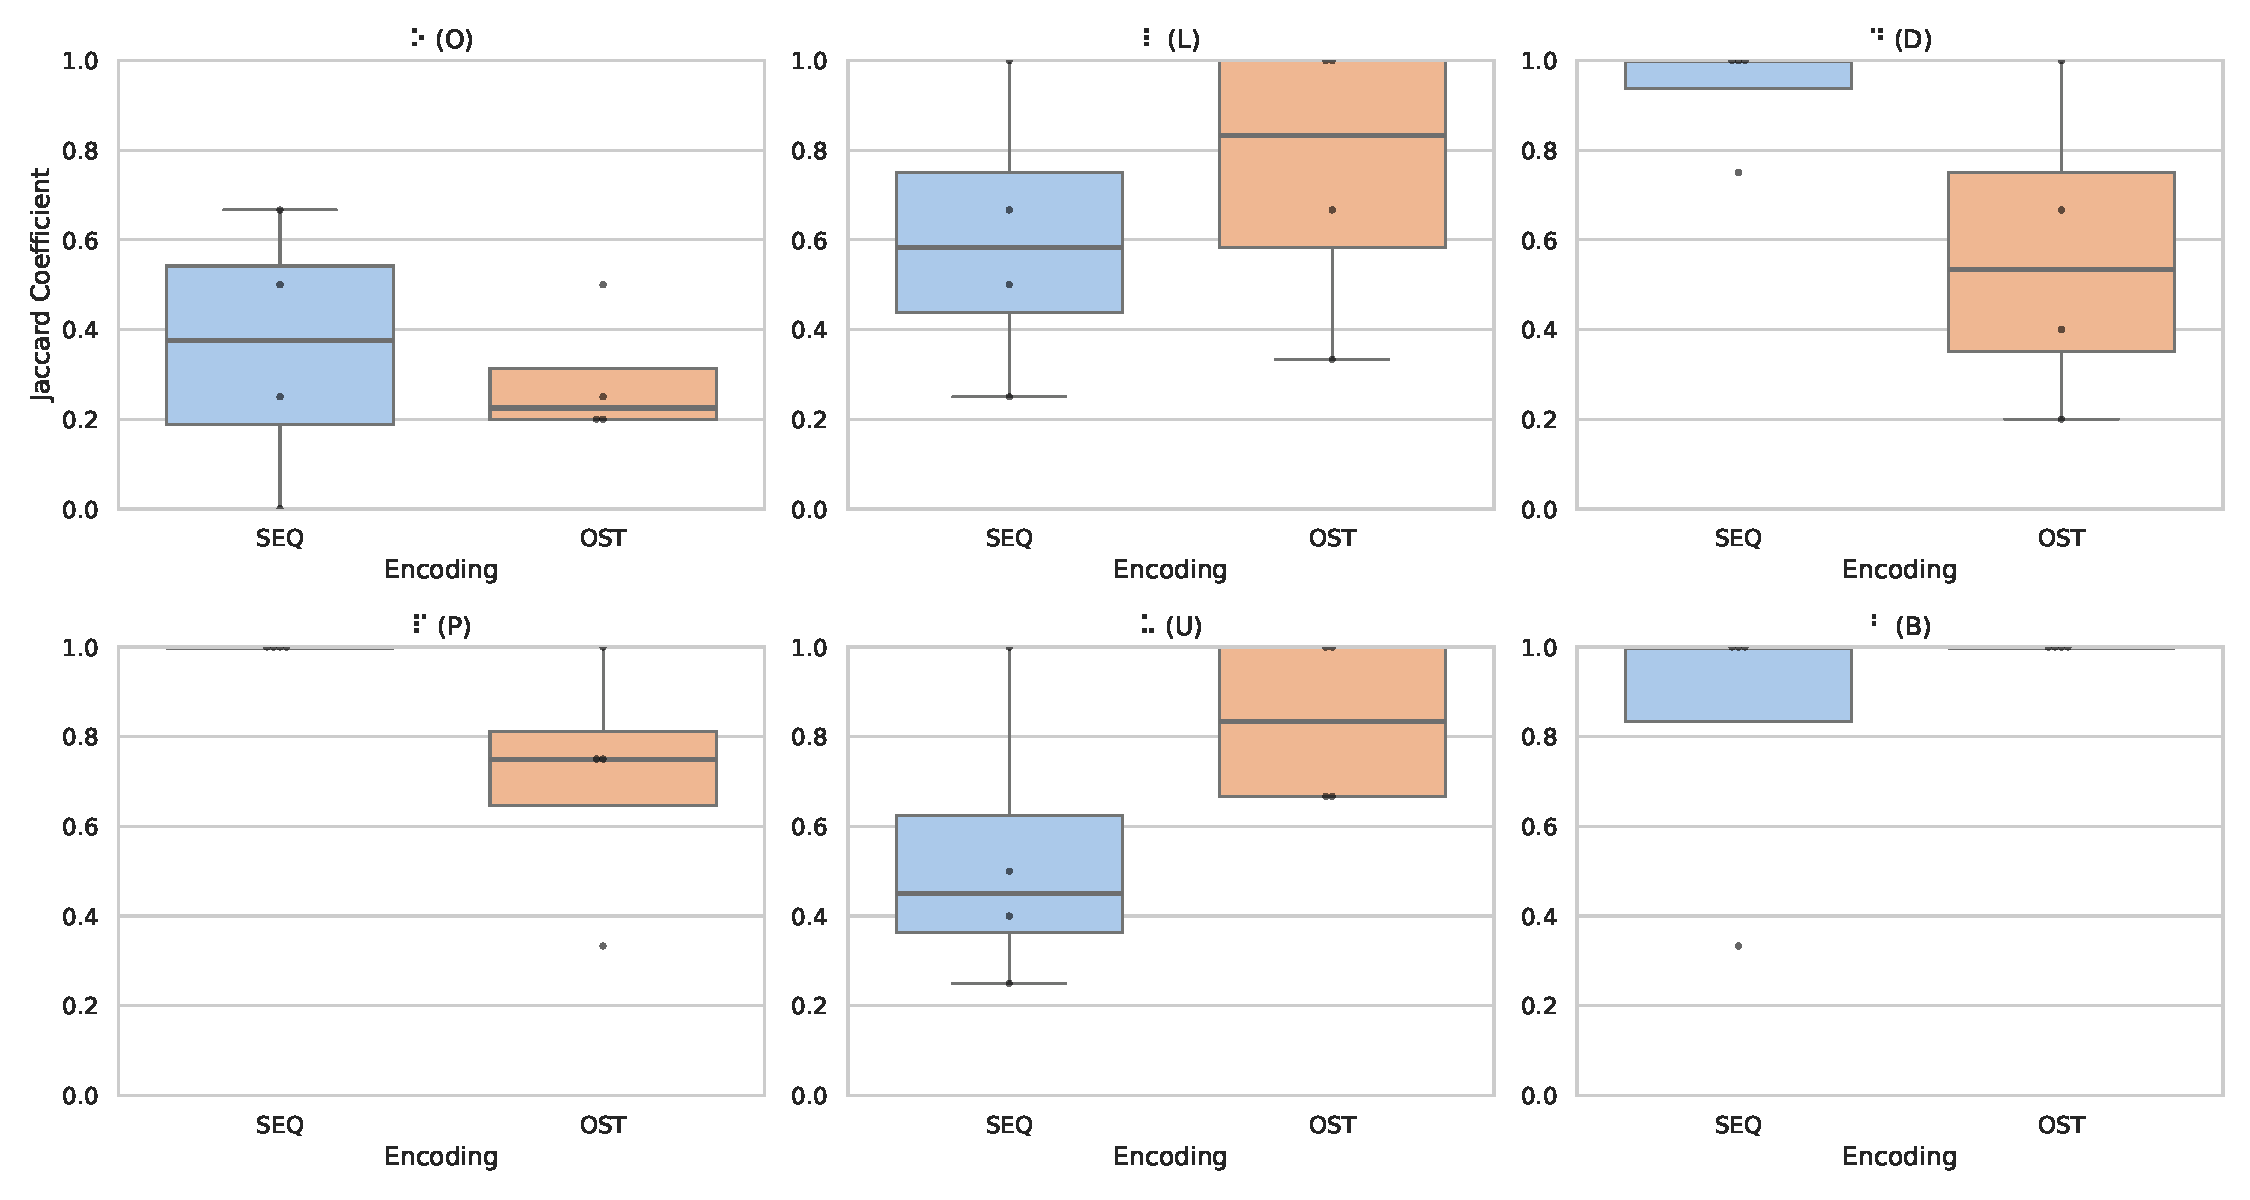
\includegraphics[width=\linewidth]{src/pictures/Study2Data_Experiment/Eval/learn_jaccard_coefficient.pdf}
    \caption{Jaccard coefficient results grouped by the Braille characters during learning for the different Encodings.}
    \label{fig:learning_results_secondStudy}
\end{figure}

During the learning process, we measured performance using the Jaccard and Dice scores. The Jaccard results after learning each character are shown in \autoref{fig:learning_results_secondStudy}, as they are more stringent than the Dice scores.

The charts reveal larger differences in the medians for \braille{d}(D), with a median of $1$ for \gls{seq} and $0.55$ for \gls{ost}.
Similarly, for the \braille{u}(U) test, the median difference is substantial, with \gls{seq} showing a median of about $0.45$ and \gls{ost} performing better with a median of $0.825$.
\gls{ost} also outperformed \gls{seq} for the character \braille{l}(L), with a median of $0.825$ compared to $0.575$ for \gls{seq}.
For the character \braille{b}(B), \gls{ost} showed better performance, with a median of $1$, which was consistent across the Q1 and Q3 quantiles. In comparison, \gls{seq} had a median of $0.825$, with Q1 equal to that value and Q3 at $1$.
However, for the character \braille{p}(P), \gls{seq} performed better, with a median, Q1, and Q3 of $1$, compared to \gls{ost}, which had a median of $0.75$, Q1 of $0.65$, and Q3 of $0.82$.

Afterwards, we conducted the appropriate \gls{mwu} tests for significance, as each user only was tested once for each character, whose results are shown in \autoref{table:learning_significance_results_secondStudy_nonPar_learning}.
However, none of the tests showed statistically significant differences.
The lowest p-value was observed in the \braille{p}(P) test, with a value of $0.067$, which also had a Cohen's d effect size of $1.492$, indicating a relatively large effect and, henceforth, indicated an approaching signifficance for the difference in the Jaccard score between the two encodings.

\begin{table}[ht]
\resizebox{\columnwidth}{!}{
\centering
\begin{tabular}{|l|l|l|l|l|}
\hline
\textbf{Question} & \textbf{Test Statistic} & \textbf{p-value}  &\textbf{Significance}           &\textbf{Effect Size}\\ \hline
\braille{o}(\textbf{O})& 10.000& 0.659&Not Significant &0.290\\ \hline
\braille{l}(\textbf{L})& 5.500& 0.552&Not Significant &0.460\\ \hline
\braille{d}(\textbf{D})& 13.500& 0.124&Not Significant &1.424\\ \hline
\braille{p}(\textbf{P})& 14.000& 0.067&Not Significant &1.492\\ \hline
\braille{u}(\textbf{U})& 3.000& 0.180&Not Significant &1.108\\ \hline
\braille{b}(\textbf{B})& 6.000& 0.453&Not Significant &0.707\\ \hline
\end{tabular}}
\caption{Results of the \gls{mwu} tests for significance grouped by the different Braille characters during training for the different Encodings with Cohen's d.}
\label{table:learning_significance_results_secondStudy_nonPar_learning}
\end{table}

\begin{figure}
    \centering
    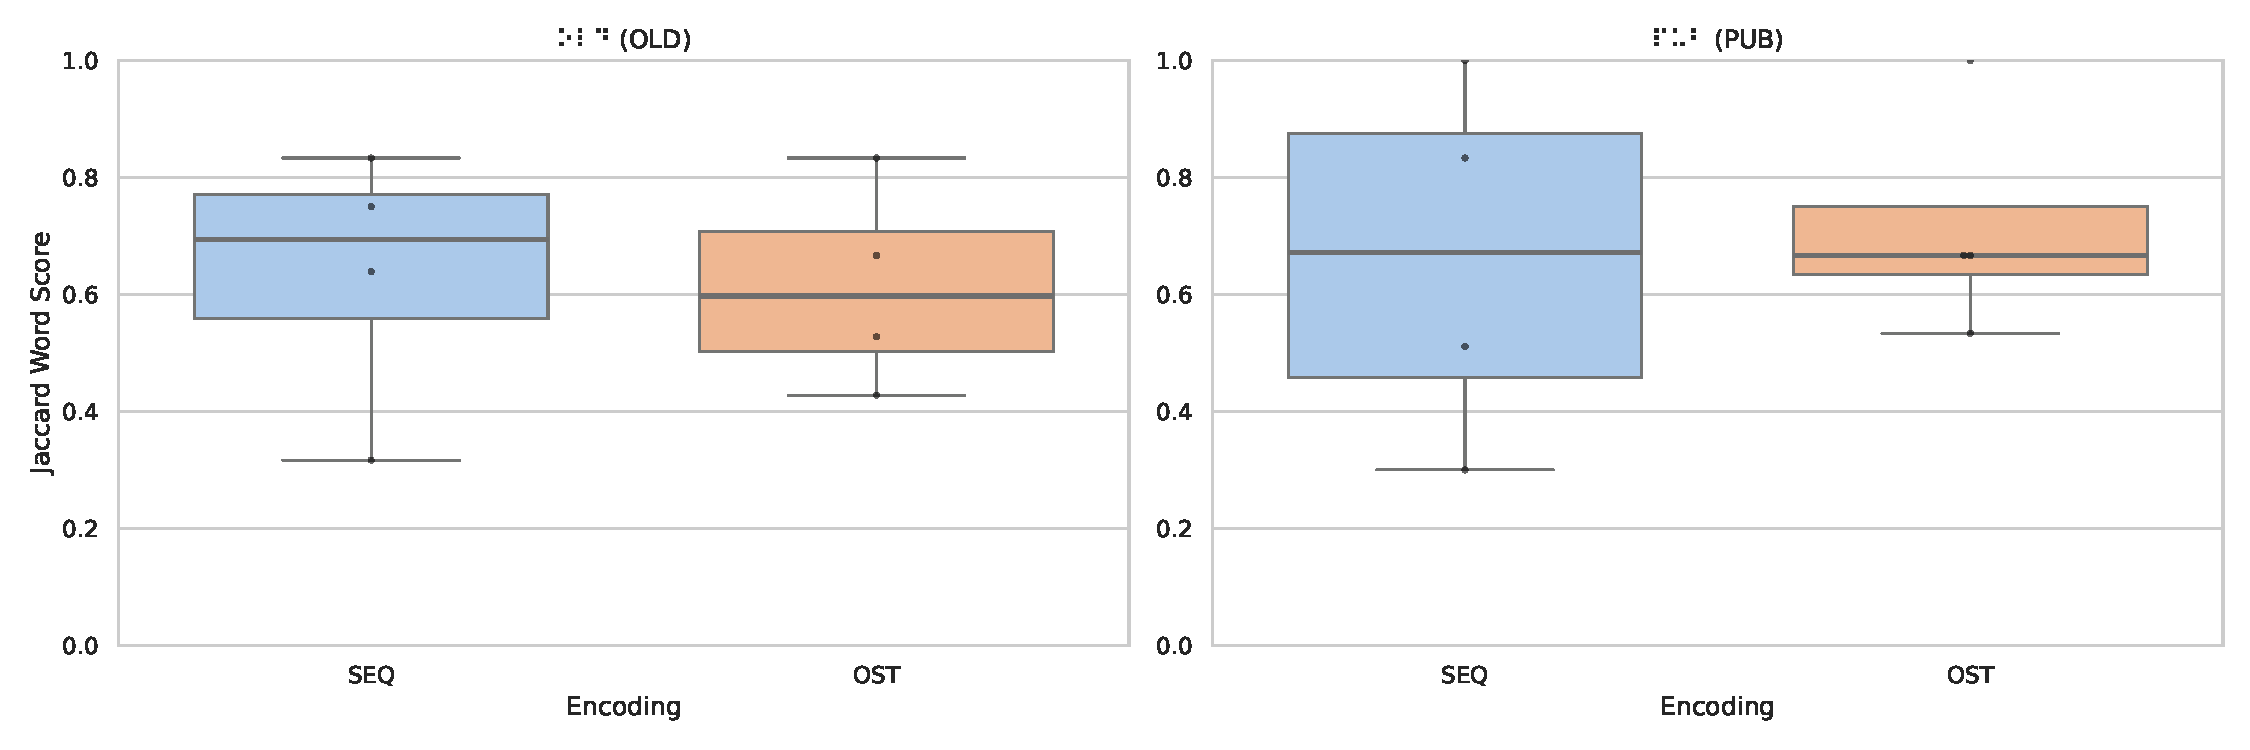
\includegraphics[width=\linewidth]{src/pictures/Study2Data_Experiment/Eval/learn_jaccard_word_score-2.pdf}
    \caption{Jaccard Word-Test results grouped by the Braille test-words for the different stimuli.}
    \label{fig:study2_test_results-firstStudy}
\end{figure}

After learning each word using one of the encodings, we tested the word itself, with the results shown in \autoref{fig:study2_test_results-firstStudy}, to determine whether there was a significant difference in testing the entire word after learning all the individual characters.
Interestingly, no significant difference was observed in the median. However, the Q1 and Q3 values for the word "pub" differed, with an interval of $0.62$-$0.85$ for \gls{ost} compared to $0.45$-$0.875$ for \gls{seq}.
Nevertheless, the median remained the same for both encodings, at $0.675$.

We conducted \gls{mwu} tests for the resulting words, and the results showed that no p-value was close to the threshold value of $0.05$, as depicted in \autoref{table:significance_results_test_secondStudy_nonPara}. This indicates that there was no significant difference between the sets, with p-values of $1.0$ and $0.77$.

\begin{table}[ht]
\resizebox{\columnwidth}{!}{
\centering
\begin{tabular}{|l|l|l|l|l|}
\hline
\textbf{Question} & \textbf{Test Statistic} & \textbf{p-value}  &\textbf{Significance}           &\textbf{Effect Size}\\ \hline
\braille{old}(\textbf{OLD})& 8.500& 1.000&Not Significant &0.103\\ \hline
\braille{pub}(\textbf{PUB})& 6.500& 0.770&Not Significant &0.211\\\hline
\end{tabular}}
\caption{Results of the \gls{mwu} tests for significance for the different Braille tests-words with a Cohens d Effect Size.}
\label{table:significance_results_test_secondStudy_nonPara}
\end{table}


\begin{figure}
    \centering
    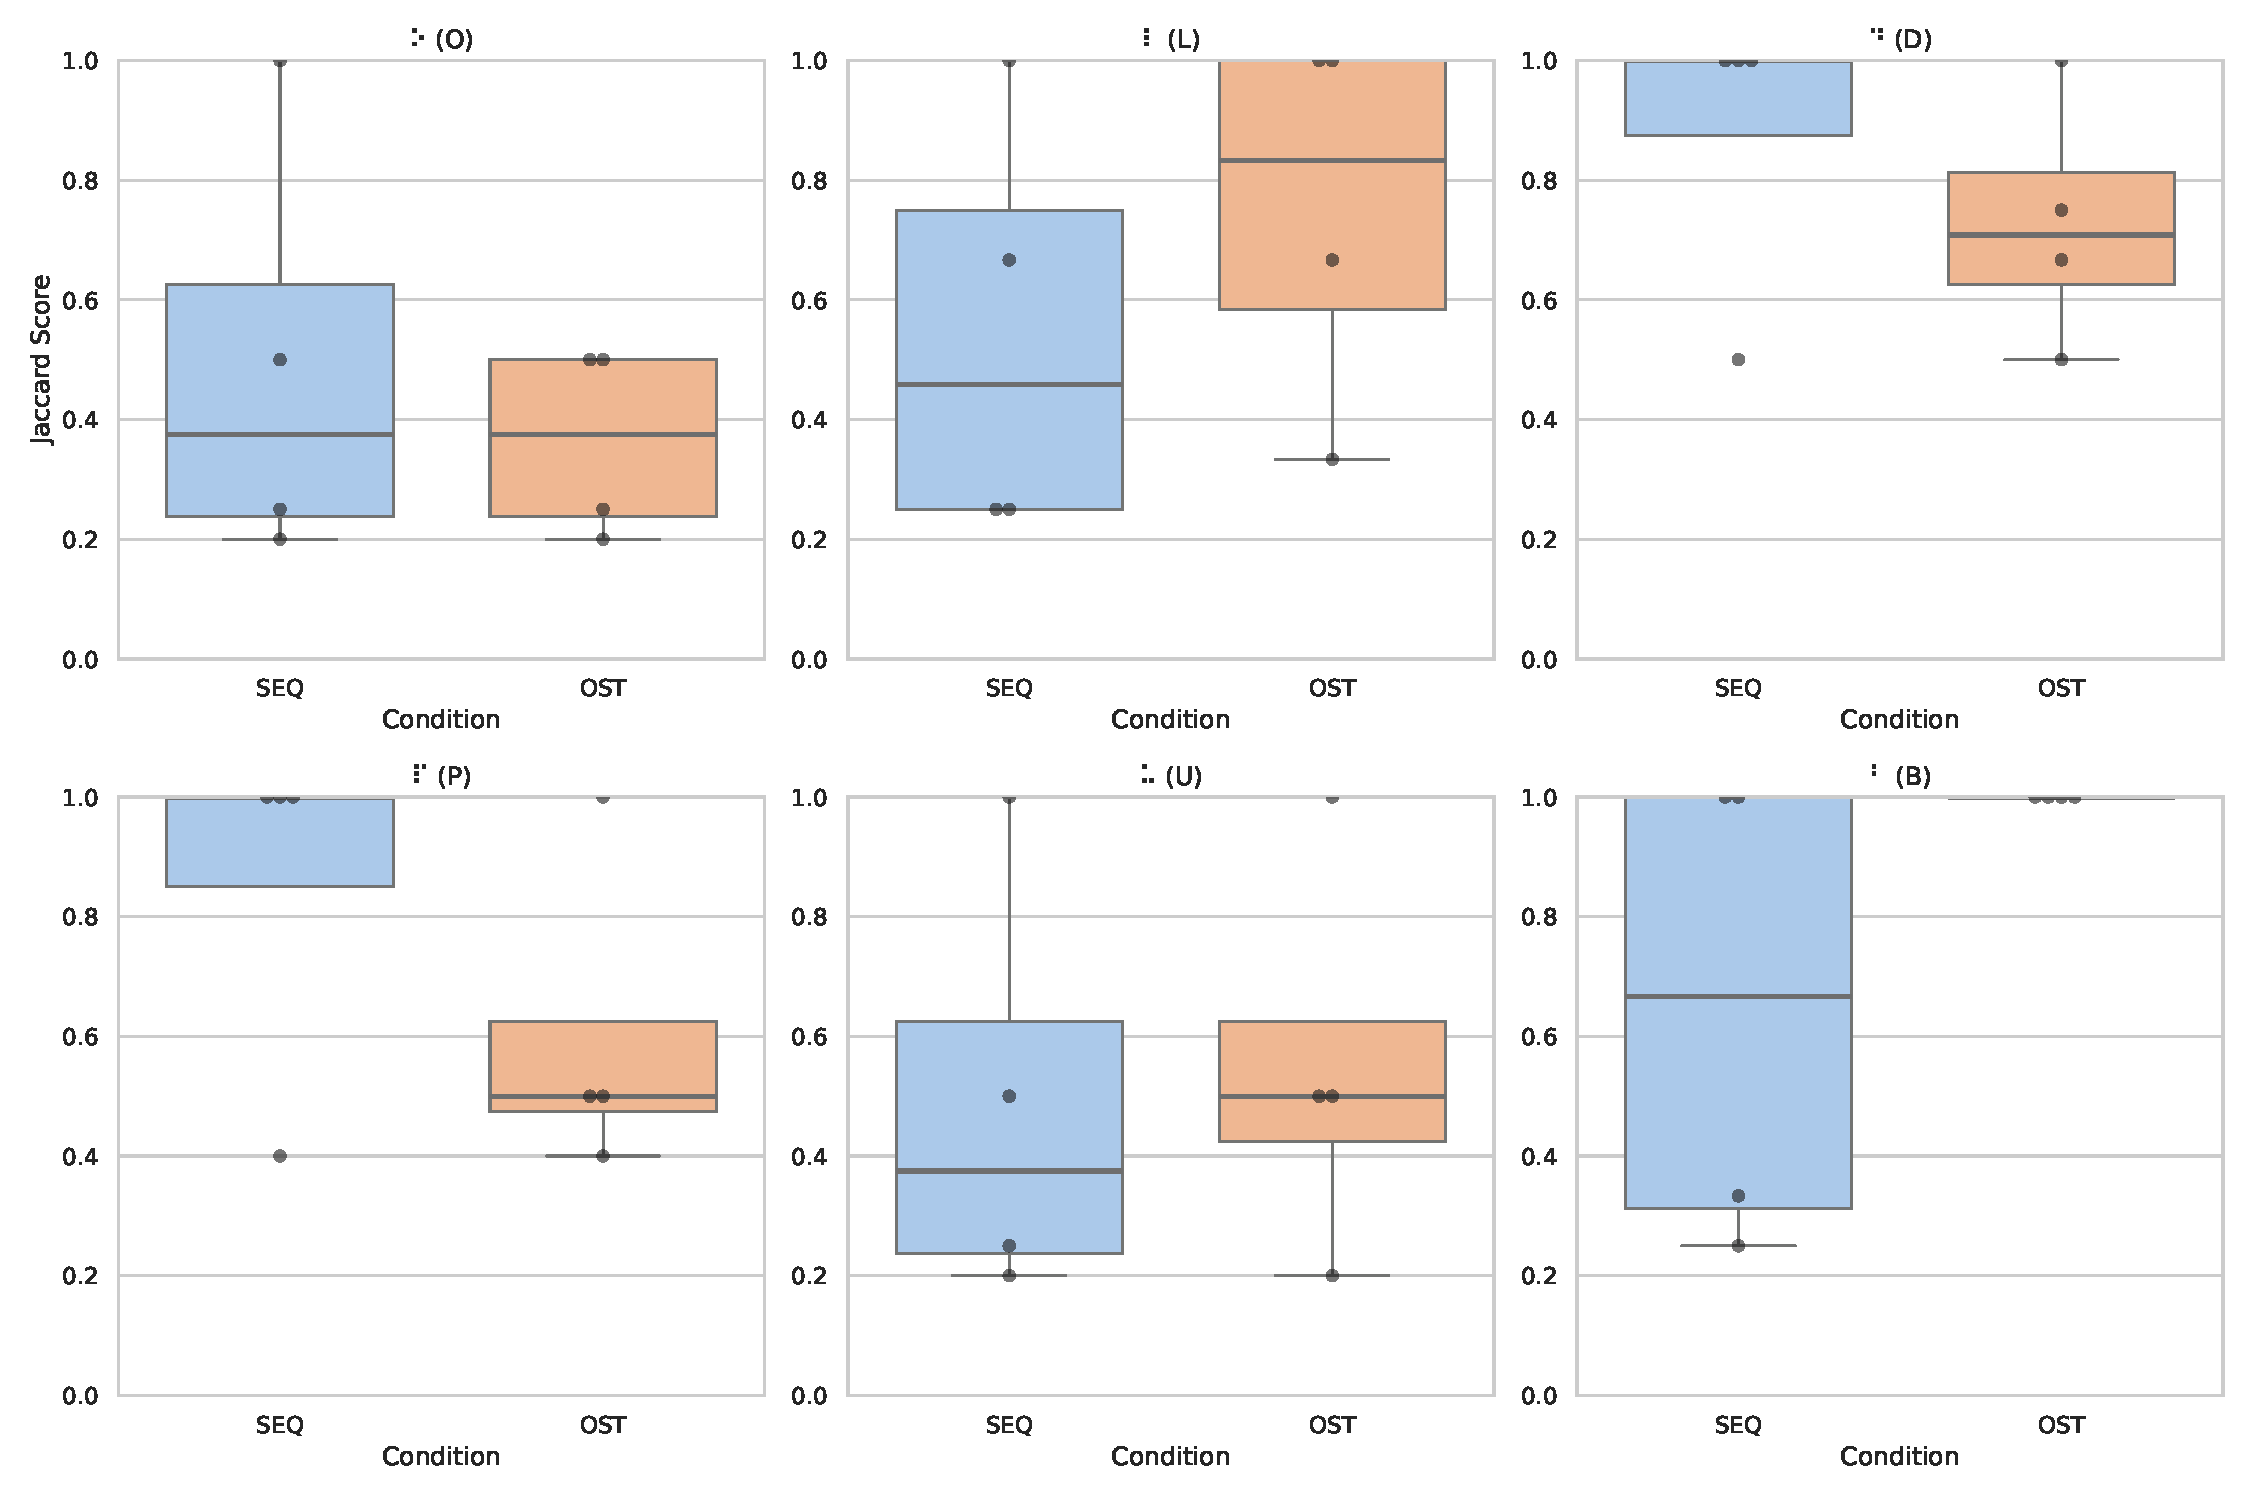
\includegraphics[width=\linewidth]{src/pictures/Study2Data_Experiment/Eval/test.pdf}
    \caption{Jaccard Score comparison for the different Encodings grouped by Braille character.}
    \label{fig:f1score_test_study2}
\end{figure}


\begin{table}[ht]
\resizebox{\columnwidth}{!}{
\centering
\begin{tabular}{|l|l|l|l|l|}
\hline
\textbf{Question} & \textbf{Test Statistic} & \textbf{p-value}  &\textbf{Significance}           &\textbf{Effect Size}\\ \hline
\braille{o}(\textbf{O})& 9.000& 0.881&Not Significant &0.443\\ \hline
\braille{l}(\textbf{L})& 4.500& 0.369&Not Significant &0.609\\ \hline
\braille{d}(\textbf{D})& 11.000& 0.439&Not Significant &0.634\\ \hline
\braille{p}(\textbf{P})& 11.000& 0.436&Not Significant &0.875\\ \hline
\braille{u}(\textbf{U})& 7.000& 0.881&Not Significant &0.179\\ \hline
\braille{b}(\textbf{B})& 4.000& 0.186&Not Significant &1.221\\ \hline
\end{tabular}}
\caption{Results of the \gls{mwu} for significance grouped by the different Braille characters during learning for the different Encodings with Cohen's d.}
\label{table:learning_significance_results_secondStudy_nonPar}
\end{table}

Similarly to the first study, we analyzed the Jaccard scores for the different characters in the second study. The most significant differences were observed for the characters \braille{b}(B), followed by \braille{p}(P), \braille{l}(L), and \braille{d}(D).

For the character \braille{b}(B), the \gls{ost} encoding performed better, achieving a perfect score, while the \gls{seq} encoding had a median of $0.675$ and a Q1-Q3 quantile range of approximately $0.3$ to $1$, as half of the participants did not achieve a perfect score.

In contrast, for the character \braille{p}(P), the \gls{ost} encoding performed worse, with a median around $0.5$, while \gls{seq} had a median of $1$. Similarly, for the character \braille{d}(D), the \gls{seq} encoding had a median of $1$, while \gls{ost} had a median of $0.7$. Notably, only one participant in the \gls{seq} group did not achieve a perfect score, with a score of $0.4$.

It is also worth noting that only one participant had a non-perfect score for \braille{d}(D) using the \gls{seq} encoding.

For the character \braille{l}(L), the \gls{ost} encoding had a median of approximately $0.825$, with half of the participants achieving a perfect score, whereas the \gls{seq} encoding had a median of about $0.45$.

Upon analyzing each character individually, no significant differences were found between the datasets. The lowest p-value was observed for \braille{b}(B), with a value of $0.186$, which is significantly higher than the threshold value. Therefore, the null hypothesis ($H_0$) cannot be rejected.

\begin{figure}
    \centering
    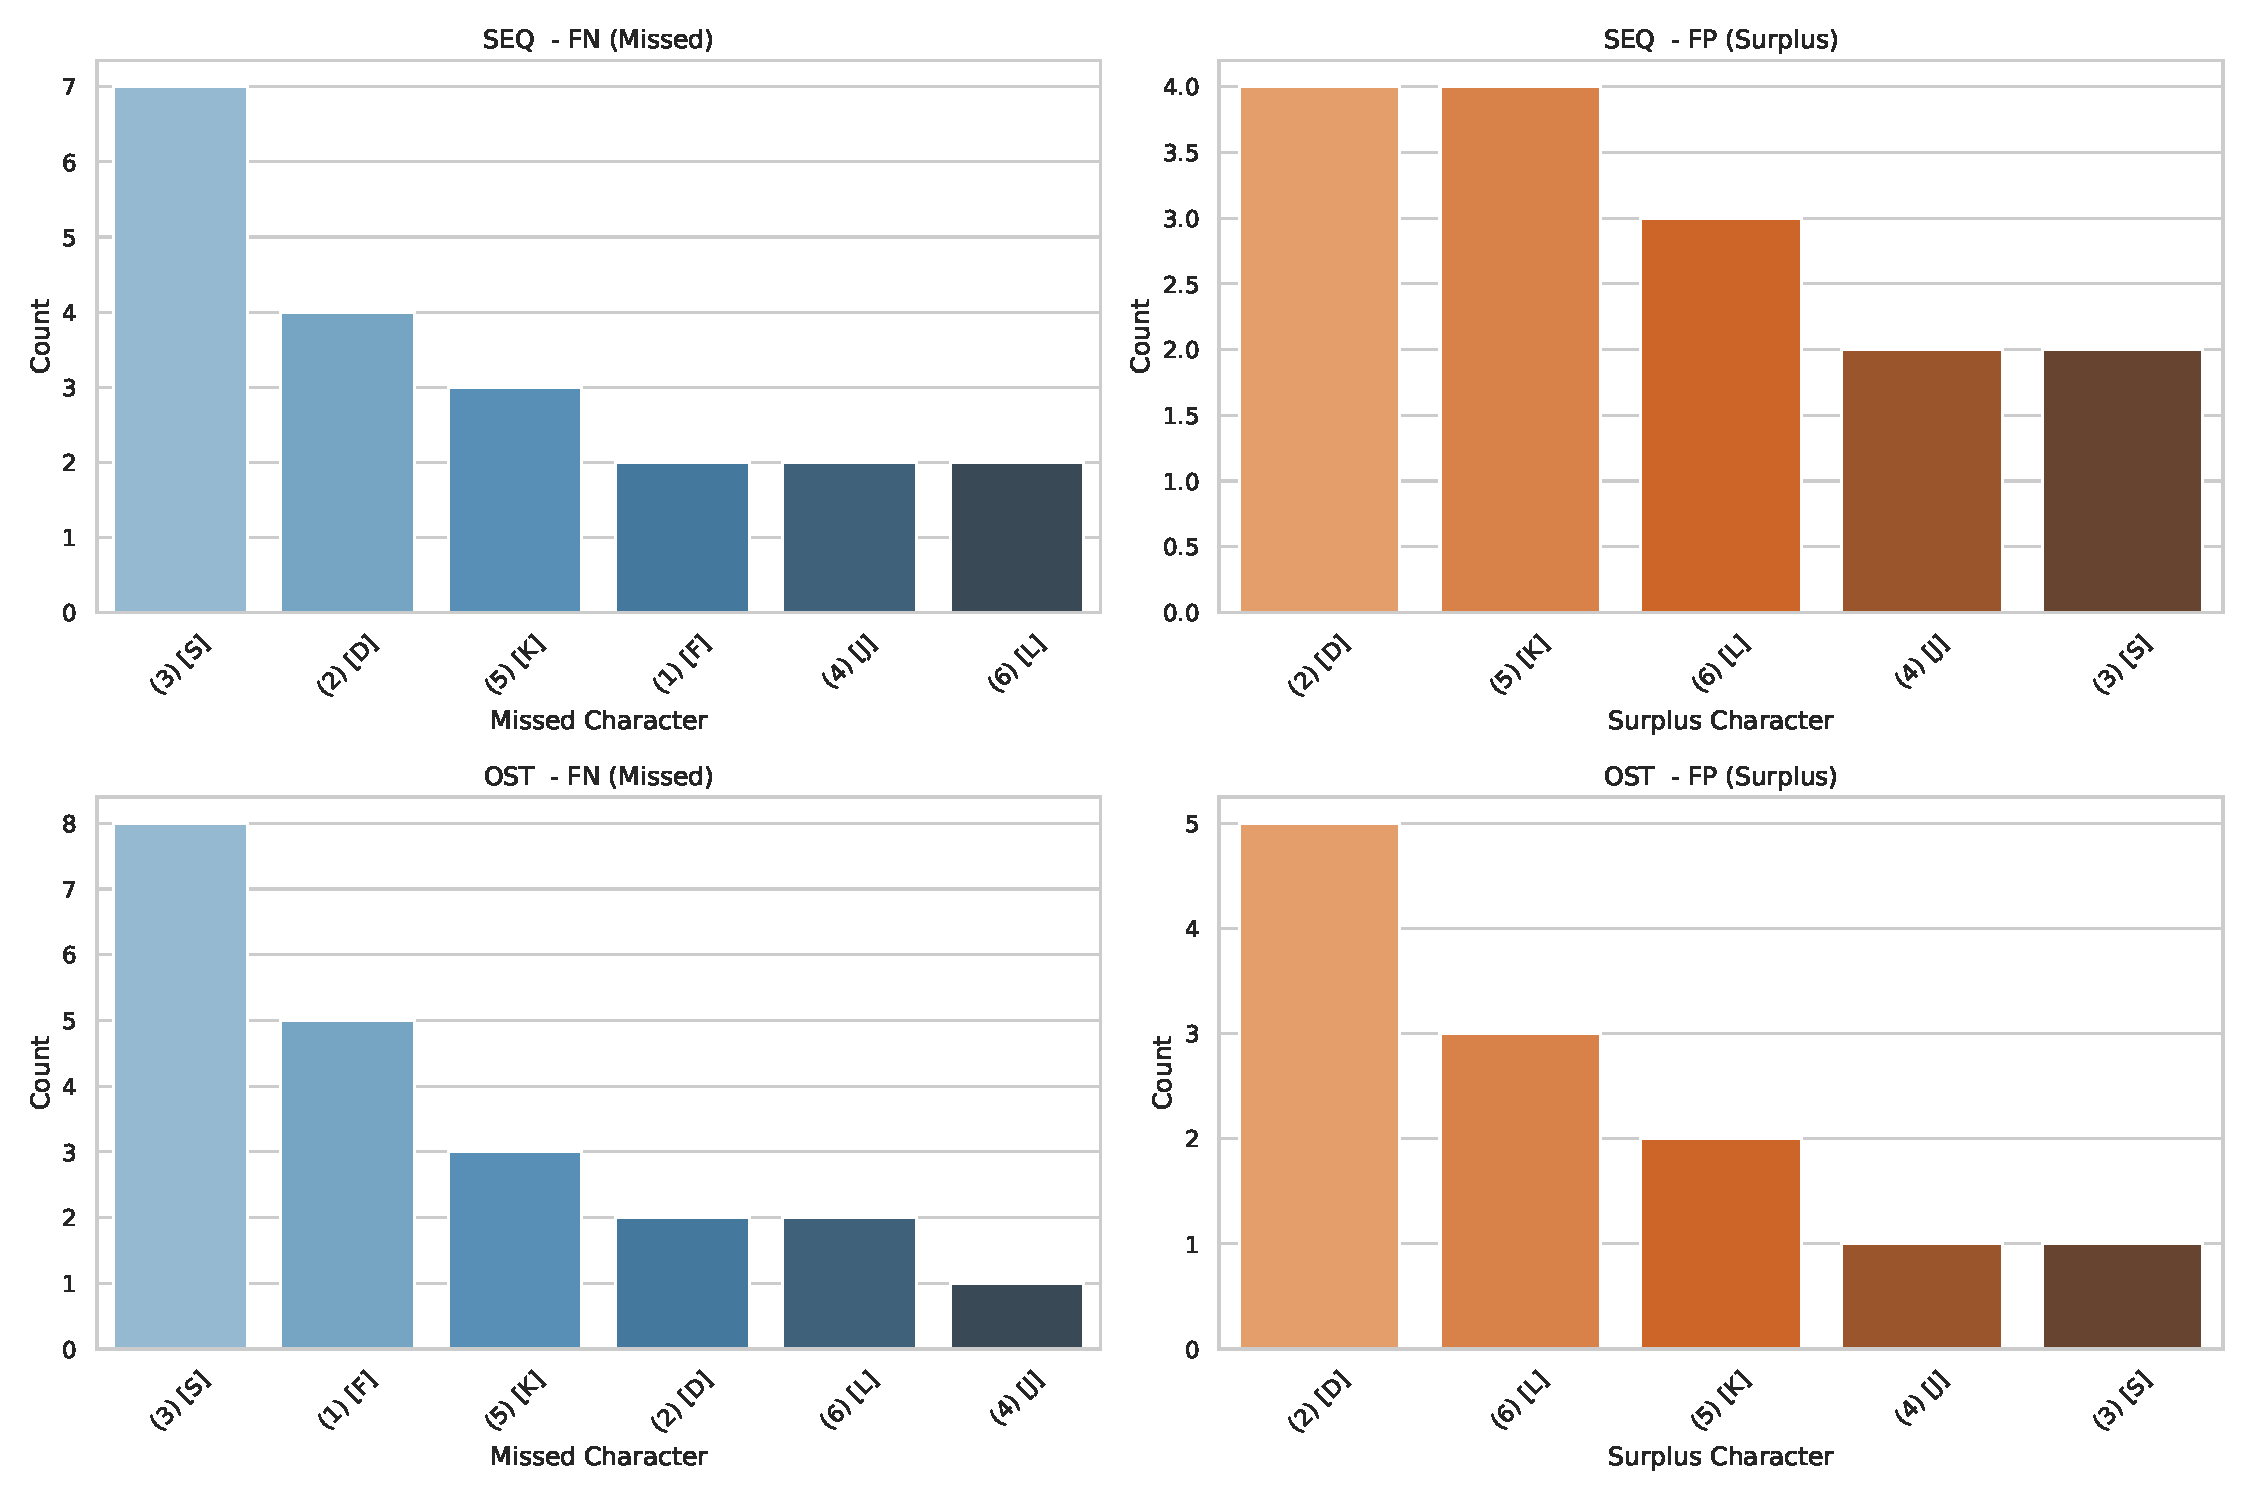
\includegraphics[width=\linewidth]{src/pictures/Study2Data_Experiment/Eval/sjkne_OST.pdf}
    \caption{FN (Missed) and FP (Surplus) Key(s) for each Braille Character by Encoding.}
    \label{fig:missedSurplus_study2}
\end{figure}

Further analysis, shown in \autoref{fig:missedSurplus_study2}, reveals that \textcircled{3} [S] is the most frequently missed character, while \textcircled{2} [D] is the most frequently in surplus. In contrast, \textcircled{4} [J] and \textcircled{6} [L] were the least missed characters, while \textcircled{2} [S] and \textcircled{4} [J] were the least in surplus.


\begin{figure}[h!]
    \centering
    \begin{subfigure}[b]{0.45\textwidth}
        \centering
        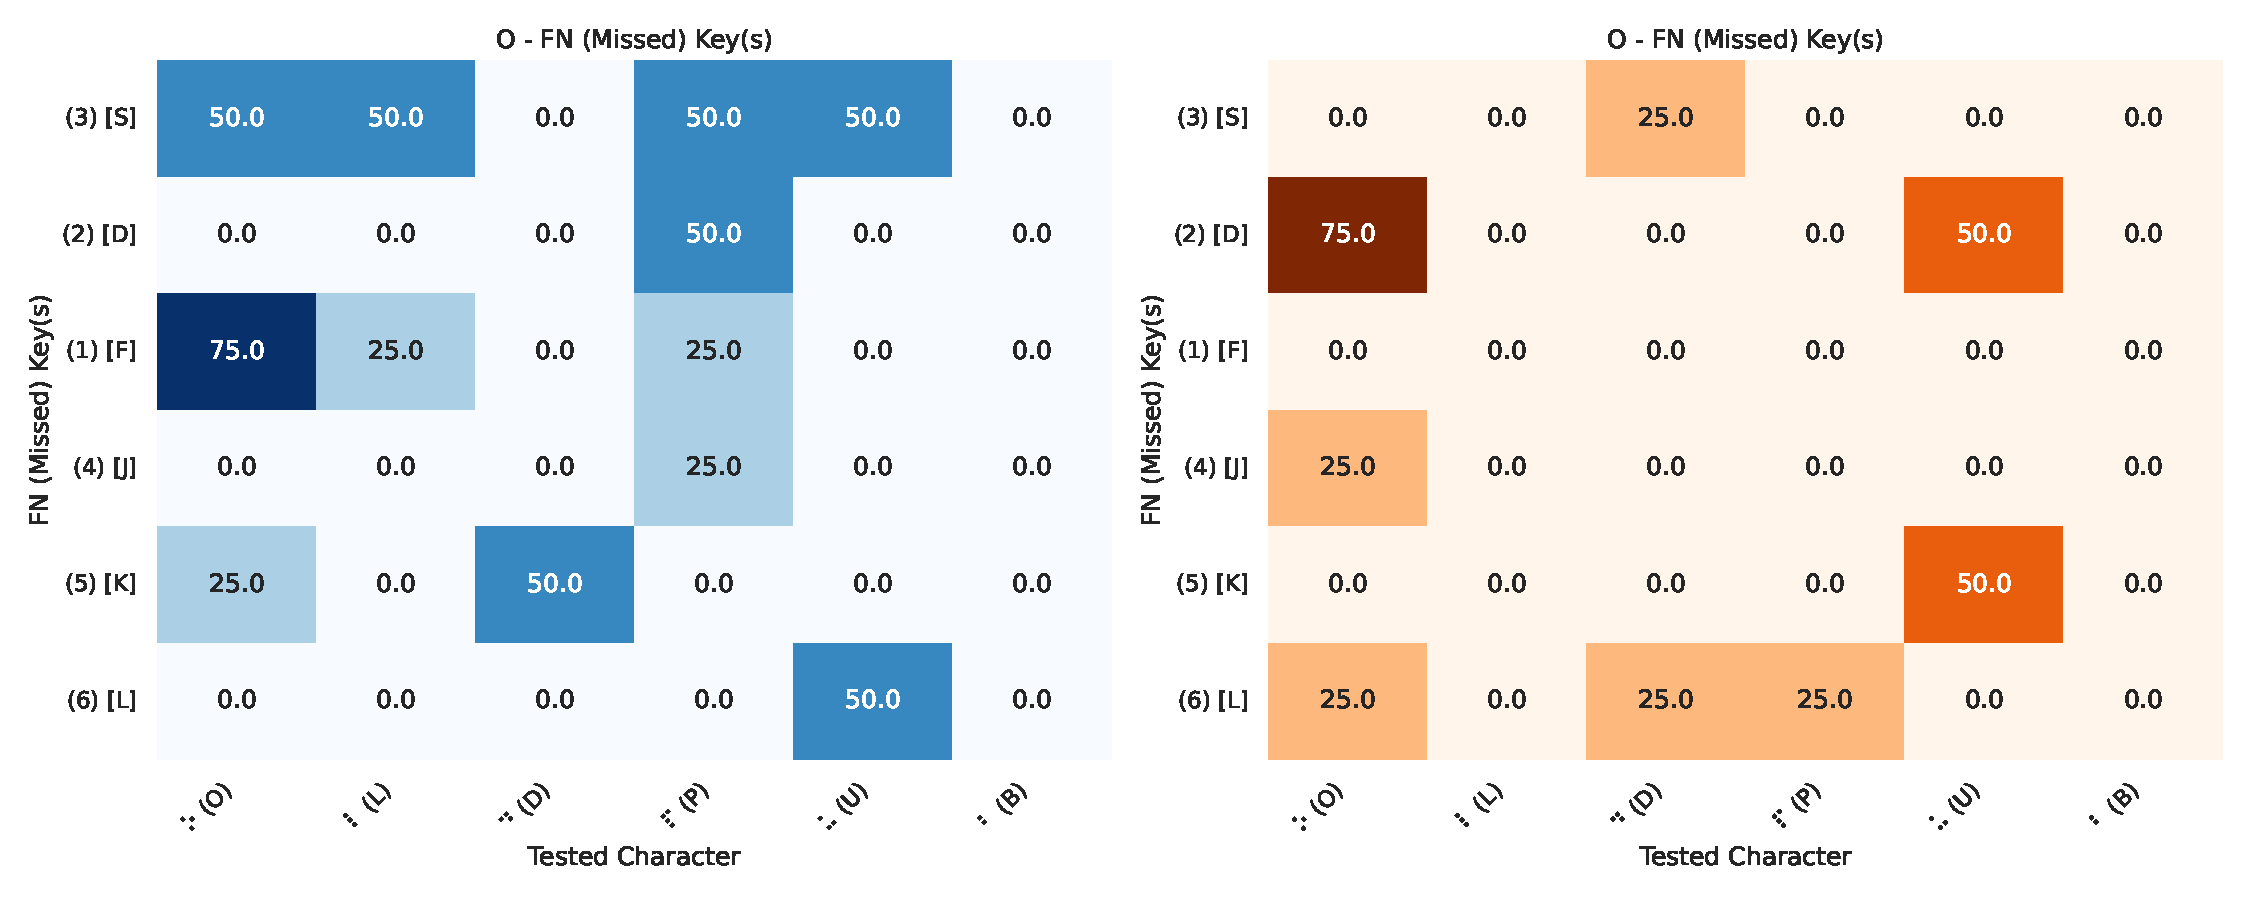
\includegraphics[width=\textwidth]{src/pictures/Study2Data_Experiment/Eval/heatmap_O_correlations_by_conditions_counts.pdf}
        \caption{\gls{ost}}
    \end{subfigure}
    \begin{subfigure}[b]{0.45\textwidth}
        \centering
        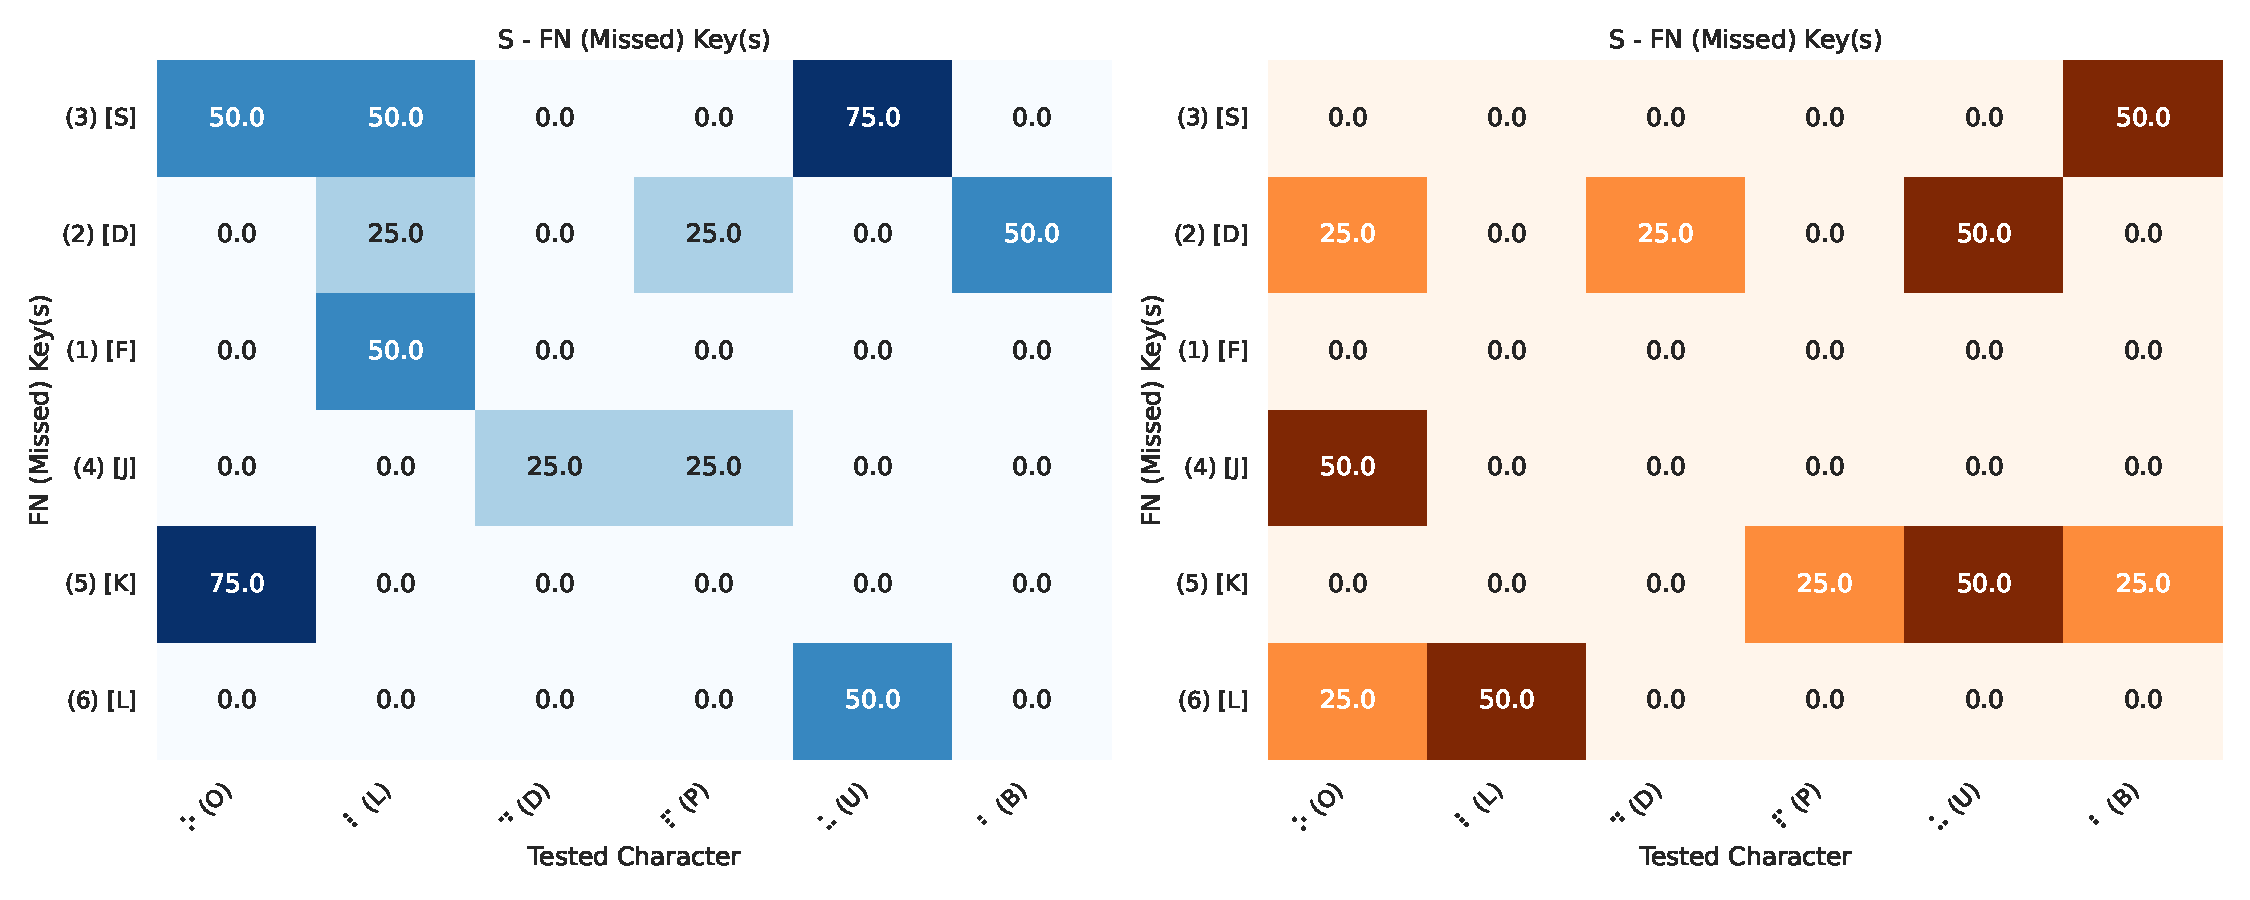
\includegraphics[width=\textwidth]{src/pictures/Study2Data_Experiment/Eval/heatmap_S_correlations_by_conditions_counts.pdf}
        \caption{\gls{seq}}
    \end{subfigure}\\
    \caption{FN (Missed) and FP (Surplus) Key(s) in percent for each Braille character grouped by Encoding.}
    \label{fig:missed_surplus_percentages_study2}
\end{figure}

A closer analysis reveals that for the false positives (FP), the characters \braille{b}(B), \braille{l}(L), \braille{d}(D), and \braille{p}(P) exhibited the most notable differences.

For \braille{b}(B), the \gls{ost} encoding had no errors, while in the \gls{seq} encoding, the \textcircled{5} [K] and \textcircled{3} [S] keys were mistakenly pressed with the \textcircled{3} [S] key in 50\% of the cases.

For \braille{l}(L), there were no false positives in the \gls{ost} encoding, but half of the participants incorrectly pressed the \textcircled{6} [L] key in the \gls{seq} encoding.

For \braille{d}(D), a larger difference is evident, with 25\% of participants missing \textcircled{3} [S] and \textcircled{6} [L] in the \gls{ost} encoding, while the \textcircled{2} [D] key was incorrectly pressed in the \gls{seq} encoding.

For \braille{p}(P), the \textcircled{6} [L] key was incorrectly pressed in 25\% of the cases in the \gls{ost} encoding, while the \textcircled{5} [K] key was mistakenly pressed in the \gls{seq} encoding.

Regarding the false negatives (FN), the most significant differences were observed for the characters \braille{p}(P), \braille{b}(B), \braille{o}(O), and \braille{l}(L). 

For \braille{p}(P), the \gls{seq} encoding performed better, with only the \textcircled{4} [J] and \textcircled{2} [D] keys missed 25\% of the time. In contrast, the \gls{ost} encoding also missed the \textcircled{1} [F] and \textcircled{3} [S] keys.

For \braille{b}(B), no keys were missed with the \gls{ost} encoding, but in the \gls{seq} encoding, the \textcircled{2} [D] key was missed 50\% of the time.

For \braille{o}(O), the \textcircled{1} [F] key was missed in 75\% of the cases with the \gls{ost} encoding, while both the \textcircled{3} [S] and \textcircled{5} [K] keys were missed in both encodings. Notably, the \textcircled{5} [K] key was missed in 75\% of the cases in the \gls{seq} encoding but only 25\% of the time in the \gls{ost} encoding.

For \braille{l}(L), both the \textcircled{1} [F] and \textcircled{3} [S] keys were missed in both encodings, though the \gls{seq} encoding also missed the \textcircled{2} [D] key 25\% of the time.

Analysis of the missed keys shows the largest differences for the \textcircled{1} [F] and \textcircled{2} [D] keys. 

The \textcircled{1} [F] key was missed in the \braille{l}(L) test in the \gls{seq} encoding, and also for \braille{o}(O) and \braille{p}(P), affecting half of the characters in the \gls{ost} encoding.

For the \textcircled{2} [D] key, it was missed for \braille{l}(L), \braille{p}(P), and \braille{b}(B) in the \gls{seq} encoding, but only in 50\% of the cases for \braille{b}(B) in the \gls{ost} encoding.

\begin{figure}
    \centering
    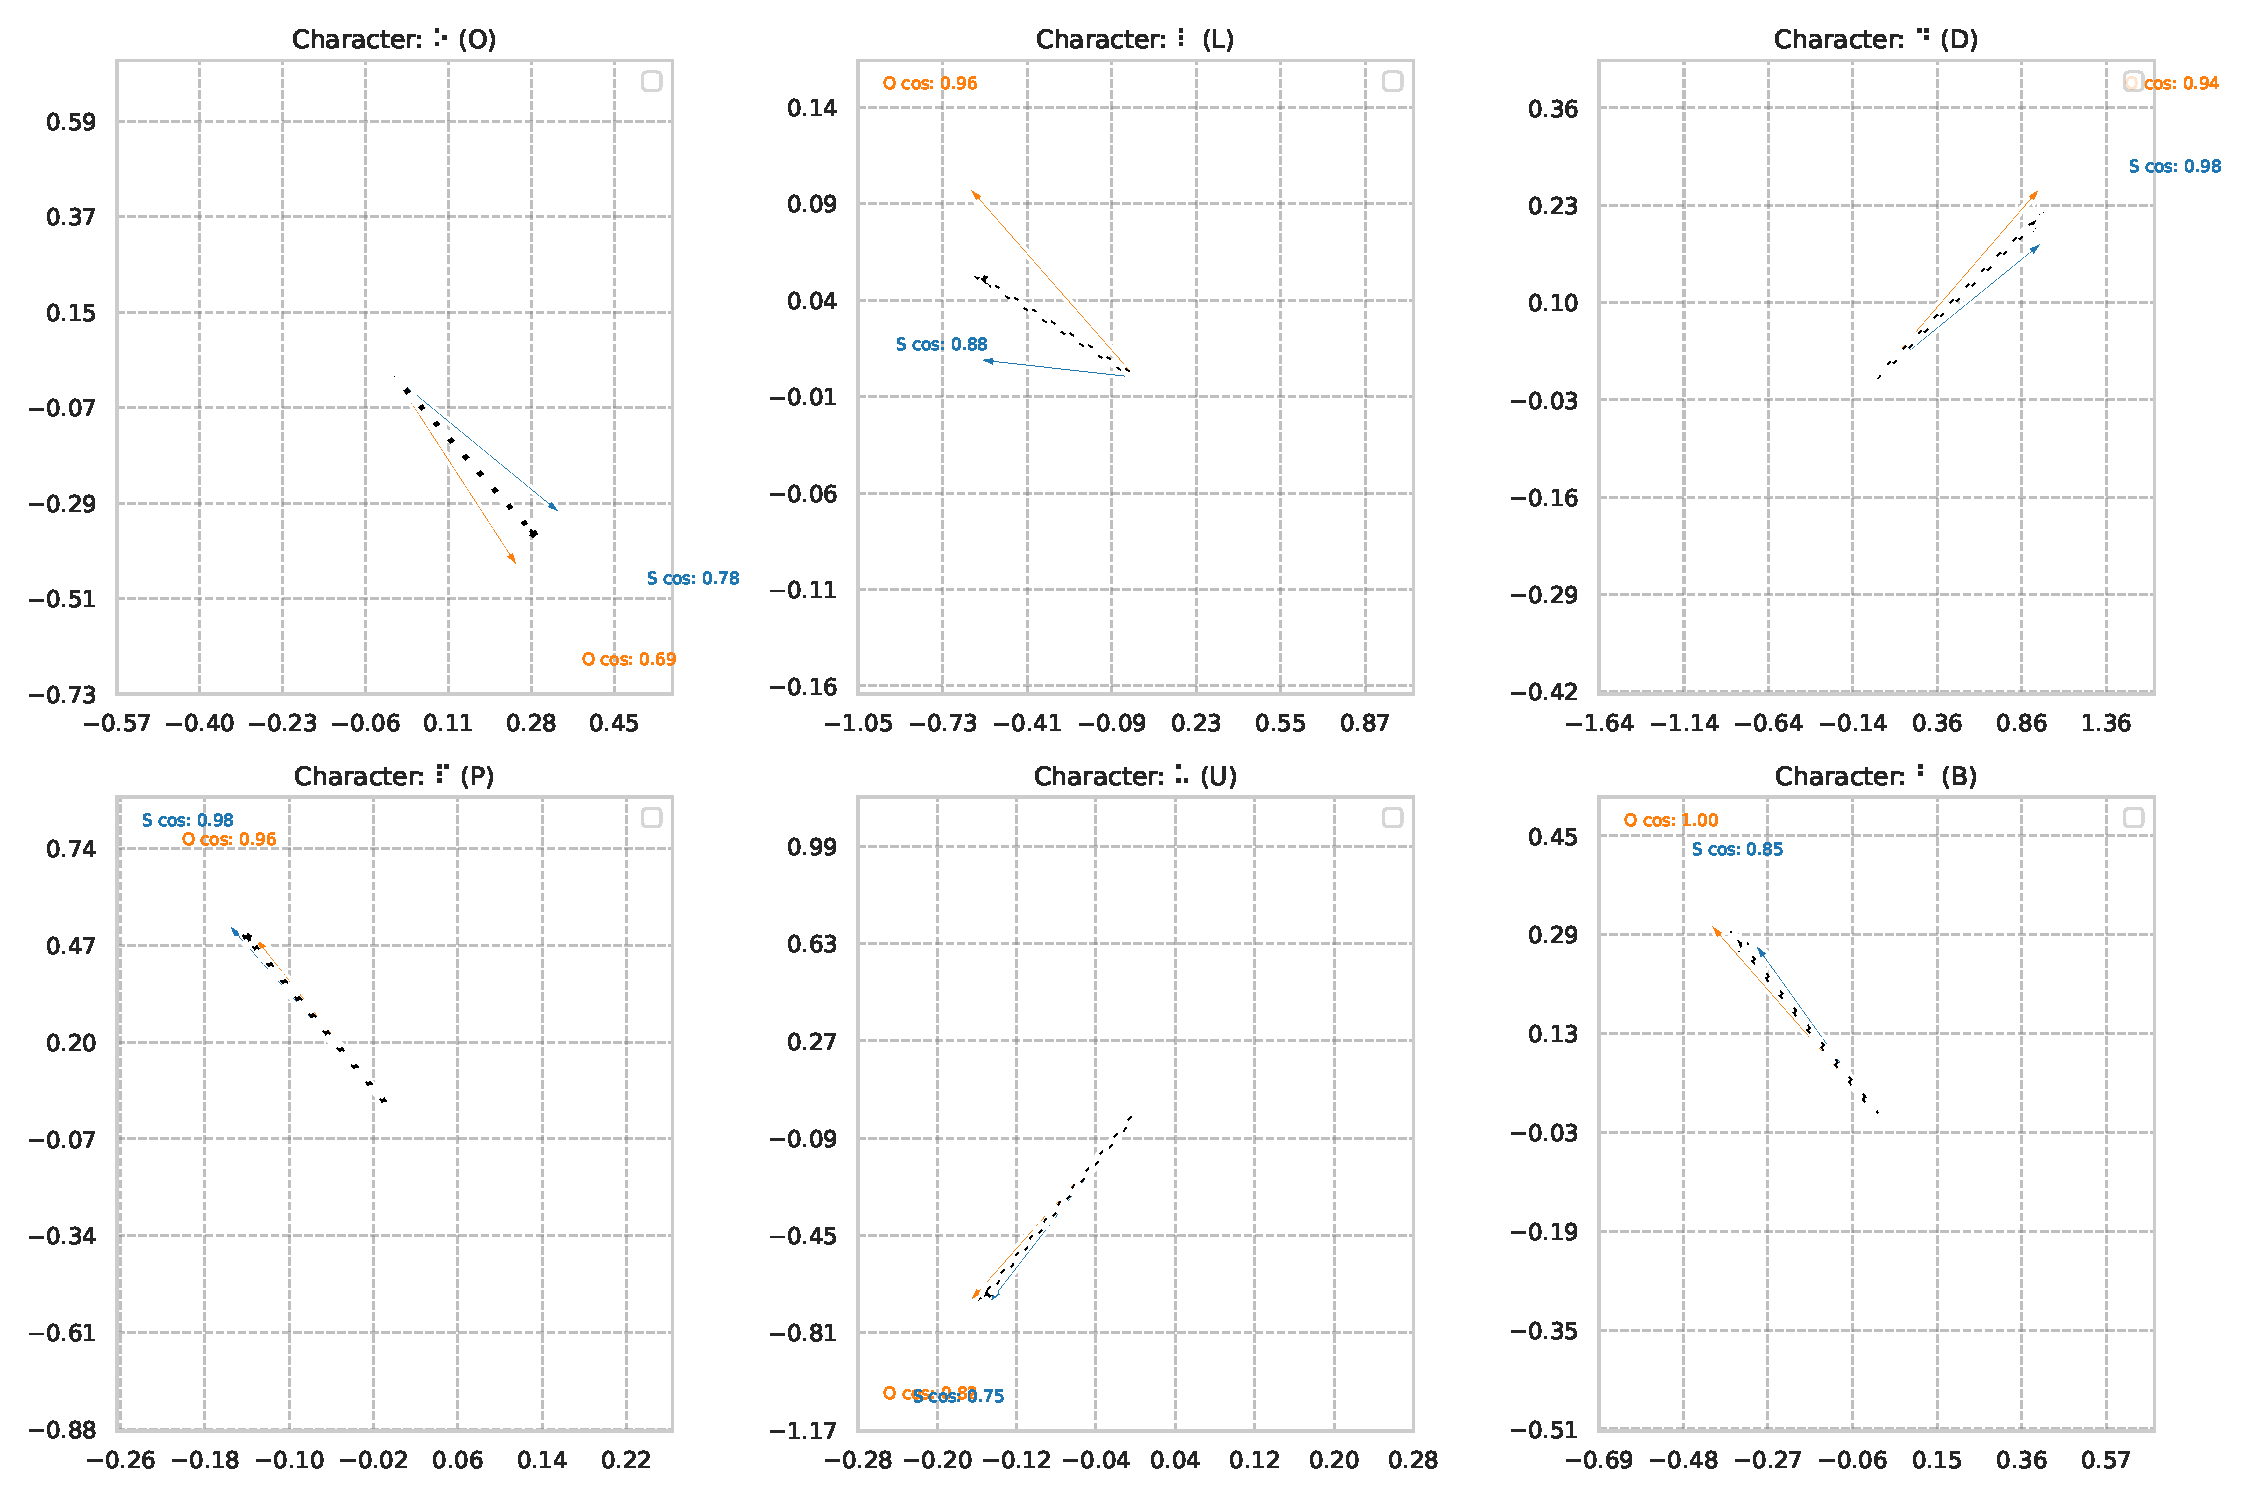
\includegraphics[width=\linewidth]{src/pictures/Study2Data_Experiment/Eval/vector.pdf}
    \caption{Cosine Similariy for each Encoding.\\Plotted using a PCA dimensionality reduction.}
    \label{fig:cosSim_PCA_study2}
\end{figure}

The cosine similarity and \gls{pca} analysis, as shown in \autoref{fig:cosSim_PCA_study2}, indicate that despite noise reduction through \gls{pca}, the vectors align in a similar direction. The most noticeable differences were observed for the braille characters \braille{o}(O) and especially \braille{l}(L).
However, their cosine similarity scores are still rather similar with 0.69 for the \gls{ost} and 0.78 for \gls{seq} for the braille character \braille{o}(O).
For the Braille character \braille{l}(L), the cosine similarity is even smaller with 0.96 for \gls{ost} and 0.88 for \gls{seq}.


\subsubsection{Questionnaire evaluation}
In our questionnaires, we analyzed correlations between individual questions to identify patterns in participants’ perceptions across the different dimensions.



\begin{table}[ht]
\resizebox{\columnwidth}{!}{
\centering
\begin{tabular}{|l|l|l|l|}
\hline
\textbf{First Question}& \textbf{Second Question}& \textbf{\gls{seq}} Pearson correlation r&\textbf{\gls{ost}} Pearson correlation r\\ \hline
Mental Demand& Physical Demand& \textbf{0.94}&\textbf{0.79}\\ \hline
& Effort& \textbf{0.96}&\textbf{0.93}\\ \hline
Effort& Frustration& \textbf{0.6}&0.38\\ \hline
& Temporal Demand& \textbf{0.88}&\textbf{0.78}\\\hline
\end{tabular}}
\caption{within NasaTLX tmp.}
\label{table:nasaTLX_correlation_secondStudy}
\end{table}

% As can be seen in the \autoref{table:nasaTLX_correlation_secondStudy} Nasatlx correlation data, there are a lot of stromg correlationds between several dimensinons.
% As depicted in the table, there is a strong correlation, that when one person has a high mental demand, for the encoding, there is also a high physical demand and effort.
% Also it can be seen for the encodings, taht a high effort correlates strongly with a high temporal demand and vice versa.
As shown in the NASA-TLX correlation data in \autoref{table:nasaTLX_correlation_secondStudy}, there are several strong correlations between various dimensions.
Specifically, the data indicates that participants who reported high mental demand during encoding also tended to report high physical demand and effort. Additionally, effort was strongly correlated with temporal demand, suggesting that participants who felt they exerted more effort also perceived the task as more time-pressured, and vice versa.

\begin{table}[ht]
\resizebox{\columnwidth}{!}{
\centering
\begin{tabular}{|l|l|l|l|}
\hline
\textbf{First Question}& \textbf{Second Question}& \textbf{\gls{seq}} Pearson correlation r&\textbf{\gls{ost}} Pearson correlation r\\ \hline
Feeling Pleasant& Helped Learning& \textbf{0.54}&\textbf{0.81}\\ \hline
& Would have learned faster& \textbf{-0.54}&\textbf{-0.75}\\ \hline
& Would use the actuators to support the learning process& 0.4&0.44\\ \hline
& Satisfaction overall& \textbf{0.55}&\textbf{0.5}\\\hline
 Helped Learning& Would have learned faster& -0.35&\textbf{-0.89}\\\hline
 & Would use the actuators to support the learning process& \textbf{0.52}&\textbf{0.72}\\\hline
 & Able to understand haptic feedback& 0.4&\textbf{0.72}\\\hline
 & Satisfaction overall& 0.31&0.49\\\hline
 Would use the actuators to support the learning process& Able to understand haptic feedback& 0.39&0.47\\\hline
 & Satisfaction overall& \textbf{0.8}&0.44\\\hline
 Would have learned faster& Would use the actuators to support the learning process& \textbf{-0.71}&-0.44\\\hline
 & Able to understand haptic feedback& 0.19&\textbf{-0.71}\\\hline
\end{tabular}}
\caption{Within Usability tmp.}
\label{table:usability_correlation_secondStudy}
\end{table}

% As can be seen in \autoref{table:usability_correlation_secondStudy}, there are high correlations within our usability questionnaire, where there each parameter has at least a moderate correlation

% Feeling Pleasant and Helped Learning is correlating with 0.54 for \gls{seq}, 0.81 and \gls{ost}, and 
% Feeling Pleasant with Would have learned faster with -0.54 for \gls{seq} and -0.75 for \gls{ost}, which shows, that if the participant  feelt pleasant, it is helping them in learning, but it's negatively correlated with that they would have learned faster without an actuator.
% Moreover we also showed, that there is a moderate correlation between Feeling pleasant and Satisfaction overall with 0.55 for \gls{seq}	and 0.5 for \gls{ost}, that shows that the participants have a higher satisfaction, when they felt pleasant and vice versa.
% Also for Helped learning and Would use the actuators to support the learning process with 0.52 for \gls{seq} and 0.72 for \gls{ost} shows that they would use the actuators again, when they felt like they helpt them in learning.
As shown in \autoref{table:usability_correlation_secondStudy}, the usability questionnaire reveals several strong correlations, with each parameter exhibiting at least a moderate correlation.
The dimensions \enquote{Feeling Pleasant} and \enquote{Helped Learning} correlate at 0.54 for \gls{seq} and 0.81 for \gls{ost}, suggesting that a more pleasant experience was associated with a stronger perception of learning support.
Additionally, \enquote{Feeling Pleasant} shows a negative correlation with \enquote{Would have learned faster without an actuator}, at -0.54 for \gls{seq} and -0.75 for \gls{ost}. This indicates that participants who felt the experience was pleasant were less likely to believe they would have learned faster without the actuator.
Furthermore, \enquote{Feeling Pleasant} also correlates moderately with \enquote{Satisfaction overall} — 0.55 for \gls{seq} and 0.50 for \gls{ost} — showing that overall satisfaction increased with the pleasantness of the experience.
Finally, the correlation between \enquote{Helped Learning} and \enquote{Would use the actuators to support the learning process} is 0.52 for \gls{seq} and 0.72 for \gls{ost}, indicating that participants who felt the actuators supported their learning would be willing to use them again.

\begin{table}[ht]
\resizebox{\columnwidth}{!}{
\centering
\begin{tabular}{|l|l|l|l|}
\hline
\textbf{First Question}& \textbf{Second Question}& \textbf{\gls{seq}} Pearson correlation r&\textbf{\gls{ost}} Pearson correlation r\\ \hline
Mental Demand& Would use the actuators to support the learning process& \textbf{-0.83}&\textbf{-0.76}\\ \hline
& Able to understand haptic feedback& -0.46&0.4\\ \hline
& Satisfaction overall& \textbf{-0.66}&0.34\\ \hline
Physical Demand& Feeling Pleasant& \textbf{0.84}&0.46\\\hline
 & Would have learned faster& -0.33&\textbf{-0.57}\\\hline
 Temporal Demand& Would use the actuators to support the learning process& \textbf{-0.79}&\textbf{-0.74}\\\hline
 & Satisfaction overall& \textbf{-0.51}&-0.37\\\hline
 Frustration& Helped Learning& -0.39&\textbf{-0.61}\\\hline
 & Would use the actuators to support the learning process& -0.42&-0.4\\\hline
 & Able to understand haptic feedback& \textbf{-0.76}&\textbf{-0.52}\\\hline
 & Satisfaction overall& -0.32&\textbf{-0.86}\\\hline
 Effort& Would use the actuators to support the learning process& \textbf{-0.7}&\textbf{-0.59}\\\hline
 & Able to understand haptic feedback& \textbf{-0.63}&-0.23\\\hline
 & Satisfaction overall& \textbf{-0.54}&\textbf{-0.52}\\\hline
 Performance& Able to understand haptic feedback& \textbf{-0.71}&-0.39\\\hline
\end{tabular}}
\caption{within between Questionnaires tmp.}
\label{table:questionnaire_correlation_secondStudy}
\end{table}
% Between the both questionnaires we found at least moderate correlation between the dimensions for the average of the both encodings and plotted them in \autoref{table:questionnaire_correlation_secondStudy}.
% As can be seen, there is a correlation of -0.83 for \gls{seq} and -0.76 for \gls{ost} for the dimensions \entquote{Mental Demand} and \entquote{Would use the actuators to support the learning process}, which shows that the higher the \entquote{mental demand} was, the lower the participants rated, that they \entquote{want to use the encoding for supporting their learning process}.
% For the dimensiosn \entquote{Temporal Demand} and \entquote{Would use the actuators to support the learning process} with a correlation of -0.79 for \gls{seq} and -0.74 for \gls{ost}, it can be seen, that there is a strong negative correlation, meaning that participant won't use the actuators to support their learning proces, if the temporal demand was high.
% Another interesting negative correlatino with -0.76 for \gls{seq} and -0.52 for \gls{ost}, for the dimensions \enquote{Frustration} and \enquote{Able to understand haptic feedback}, shows that there is a negative correlatino with the participants able to understand the feedback and being frustrated.
% We found other at least moderate correlations for the dimensions \enquote{Effort} and \enquote{Would use the actuators to support the learning process} with a moderate negative correlation of \textbf{-0.7}	\textbf{-0.59}
% for \gls{ost} and \gls{seq} respectively and \enquote{Effort} and \enquote{Satisfaction overall} with a negative correlation of \textbf{-0.54}	and \textbf{-0.52} for \gls{seq} and \gls{ost} respectively.
% Both show, that when the effort was high, the participants would rather not use those actuators to support the learning efforts and their satisfaction was also more negative and vice versa.
Across both questionnaires, we identified several dimension pairs with at least moderate correlations for the average values of the two encodings, as shown in \autoref{table:questionnaire_correlation_secondStudy}.
Notably, there is a strong negative correlation between \enquote{Mental Demand} and \enquote{Would use the actuators to support the learning process}, with values of -0.83 for \gls{seq} and -0.76 for \gls{ost}. This suggests that higher perceived mental demand was associated with a lower willingness to use the actuator-based encoding in future learning scenarios.
Similarly, \enquote{Temporal Demand} and \enquote{Would use the actuators to support the learning process} show strong negative correlations of -0.79 for \gls{seq} and -0.74 for \gls{ost}, indicating that participants who experienced high time pressure were less inclined to use the actuators again.
Another noteworthy finding is the negative correlation between \enquote{Frustration} and \enquote{Able to understand haptic feedback}, with values of -0.76 for \gls{seq} and -0.52 for \gls{ost}. This implies that increased frustration was associated with a lower perceived ability to understand the haptic feedback.
Additional moderate correlations were found between \enquote{Effort} and \enquote{Would use the actuators to support the learning process}, with values of -0.70 for \gls{ost} and -0.59 for \gls{seq}, as well as between \enquote{Effort} and \enquote{Satisfaction overall}, at -0.54 for \gls{seq} and -0.52 for \gls{ost}. These results indicate that higher perceived effort was linked to both lower satisfaction and reduced willingness to use the actuators for learning support.


\subsubsection{User comments}
We analysed the user comments, on their free form section in the questionnaire to see what their comments are between teh encoding schemes and they were:
\enquote{For OST, I don't perceive the vibration as accurately.},
\enquote{I had difficulties to register which finger did vibrate.},
\enquote{If I had to learn with one method with the goal of having learned something in the end, I would choose SEQ. If it's just for fun, I would choose OST.},
\enquote{I had difficulties to register which finger did vibrate.},
\enquote{OST was easier to ignore. SEQ was harder to ignore, more irritating during the game.},
\enquote{In the second section, I learned the Braille better because the devices of each finger didn’t vibrate at the same time.},
This shows that the users seem to prefer the \gls{seq} encoding over the \gls{ost} by saying it is more distinguishable.





\section{Threats to Validity}

We identified several potential threats to validity in both of our studies, which are categorized into internal, external, and construct validity, following the framework outlined by Lago et al. \cite{10.1145/3674805.3686691} which are illustrated in \autoref{fig:threats_to_validity}.

\subsection{Internal Validity}
% One key threat to internal validity is the sample size. In the \textbf{first study}, an \textit{a priori} power analysis using the g* power software determined that a sample size of \textbf{36} was required to achieve \textbf{80\% power}. However, only \textbf{12} samples were used, and a \textit{post hoc} power analysis revealed an achieved power of only \textbf{0.34}. This low statistical power increases the risk of a \textbf{Type II error}, meaning that true effects may not have been detected. 

% Similarly, in the \textbf{second study}, the \textit{a priori} power analysis indicated that a sample size of \textbf{45} was necessary for adequate statistical power. However, the \textit{post hoc} power analysis showed that the actual power achieved was only \textbf{0.356}. These findings suggest that both studies were underpowered, limiting the reliability of their conclusions.
One key threat to internal validity in this research is the insufficient sample size. In the first study, an \textit{a priori} power analysis using the G*Power software indicated that a sample size of 43 participants was necessary to detect an effect size of 0.25 with 80\% power at an alpha level of 0.05. However, only 12 participants were recruited, and a \textit{post hoc} power analysis revealed an actual power of just 40.86\%. 

Similarly, in the second study, a total of 54 participants were required for the same effect size and significance level, but only 8 were included, resulting in an achieved power of merely 23.21\%. 

Both studies were therefore underpowered with an power level lower than 80\%.


Additionally, we used a relatively young participant group, with a median age of 28.67 years in the first study and 24.5 years in the second study. Both studies also included only one left-handed participant. Furthermore, the gender distribution was imbalanced, with only three female participants in each study. This lack of diversity may limit the generalizability of our findings across different populations.

\subsection{External and Construct Validity}
Hand size emerged as a potential factor affecting external and construct validity. Differences in hand size may influence the placement of actuators, as they could sit differently on individuals with larger or smaller hands. This variation in actuator positioning could have introduced slight inconsistencies in the stimuli delivered, potentially influencing our results.

Another construct validity concern relates to stimulus perception. Some participants reported that they did not perceive the stroking stimulus as effectively as the vibration or tapping stimuli. This perception discrepancy could impact the interpretation of the stimulus' effects and must be considered when evaluating the results.

Lastly, none of the participants were native English speakers. Although the words used in the experiments were simple, short, and commonly encountered, some participants may have had minor spelling difficulties. However, we consider this issue to have a negligible impact on the findings.

\begin{figure}
    \centering
    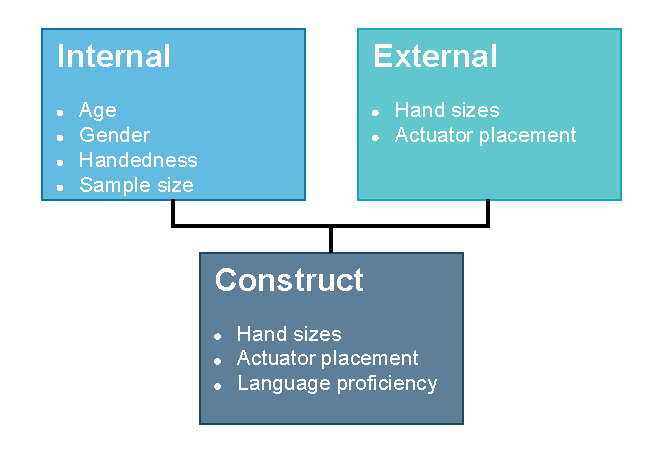
\includegraphics[width=0.5\linewidth]{src/pictures/StudyData/Threats_to_validity.drawio.pdf}
    \caption{Threats to validity}
    \label{fig:threats_to_validity}
\end{figure}


